\documentclass[11pt,a4paper,oneside]{report}
\usepackage[a4paper,margin=25mm,headheight=15pt,footskip=12mm]{geometry}
\usepackage[T1]{fontenc}
\usepackage[utf8]{inputenc}
\usepackage{lmodern}
\usepackage{microtype}
\usepackage{graphicx}
\usepackage{booktabs,tabularx,longtable,array}
\usepackage{amsmath,amssymb}
\usepackage{tikz}
\usetikzlibrary{arrows.meta,positioning,fit,calc}
\usepackage{xcolor}
\usepackage{caption,subcaption}
\usepackage{fancyhdr}
\usepackage{titlesec}
\usepackage{enumitem}
\usepackage{listings}
\usepackage{hyperref}
\usepackage{xurl}
\usepackage{url}
\usepackage{float}
\usepackage{needspace}
\definecolor{ink}{HTML}{172B36}
\definecolor{teal}{HTML}{087E78}
\definecolor{muted}{HTML}{526873}
\definecolor{rulegray}{HTML}{D5DEE2}
\definecolor{papergray}{HTML}{F3F6F6}
\hypersetup{colorlinks=true,linkcolor=teal,urlcolor=teal,citecolor=teal,pdftitle={Orbit SIS: System Design and Verification Report},pdfauthor={System Design Lab},pdfsubject={Student information system architecture and verification}}
\setlength{\parindent}{0pt}
\hyphenpenalty=10000
\exhyphenpenalty=10000
\setlength{\parskip}{5pt plus 1pt}
\setlist[itemize]{leftmargin=1.5em,itemsep=2pt,topsep=3pt}
\setlist[enumerate]{leftmargin=1.7em,itemsep=3pt,topsep=3pt}
\renewcommand{\arraystretch}{1.2}
\captionsetup{font=small,labelfont=bf,labelsep=period,justification=raggedright,singlelinecheck=false}
\titleformat{\chapter}[display]{\normalfont\bfseries\color{ink}}{\large\color{teal}\chaptername\ \thechapter}{7pt}{\Huge}
\titlespacing*{\chapter}{0pt}{-18pt}{18pt}
\titleformat{\section}{\Large\bfseries\color{ink}}{\thesection}{0.7em}{}
\titleformat{\subsection}{\large\bfseries\color{teal}}{\thesubsection}{0.7em}{}
\pagestyle{fancy}\fancyhf{}
\fancyhead[L]{\small\textsc{Orbit SIS} \; / \; System design}
\fancyhead[R]{\small\nouppercase{\leftmark}}
\fancyfoot[L]{\small Engineering case study · 21 October 2026}
\fancyfoot[R]{\small\thepage}
\renewcommand{\headrulewidth}{0.4pt}\renewcommand{\footrulewidth}{0pt}
\begin{document}
\begin{titlepage}
\thispagestyle{empty}
\color{ink}
\vspace*{8mm}
{\large\color{teal}\textsc{SYSTEM DESIGN LAB}}\par
\vspace{5mm}
\rule{\linewidth}{1.1pt}\par
\vspace{7mm}
{\fontsize{28}{34}\selectfont\bfseries Designing a Student Information\\System Around Correctness}\par
\vspace{5mm}
{\Large\color{muted}Architecture, transactional enrollment, and evidence-based verification}\par
\vspace{4mm}
\begin{center}
\setlength{\fboxsep}{2pt}
\color{rulegray}\fbox{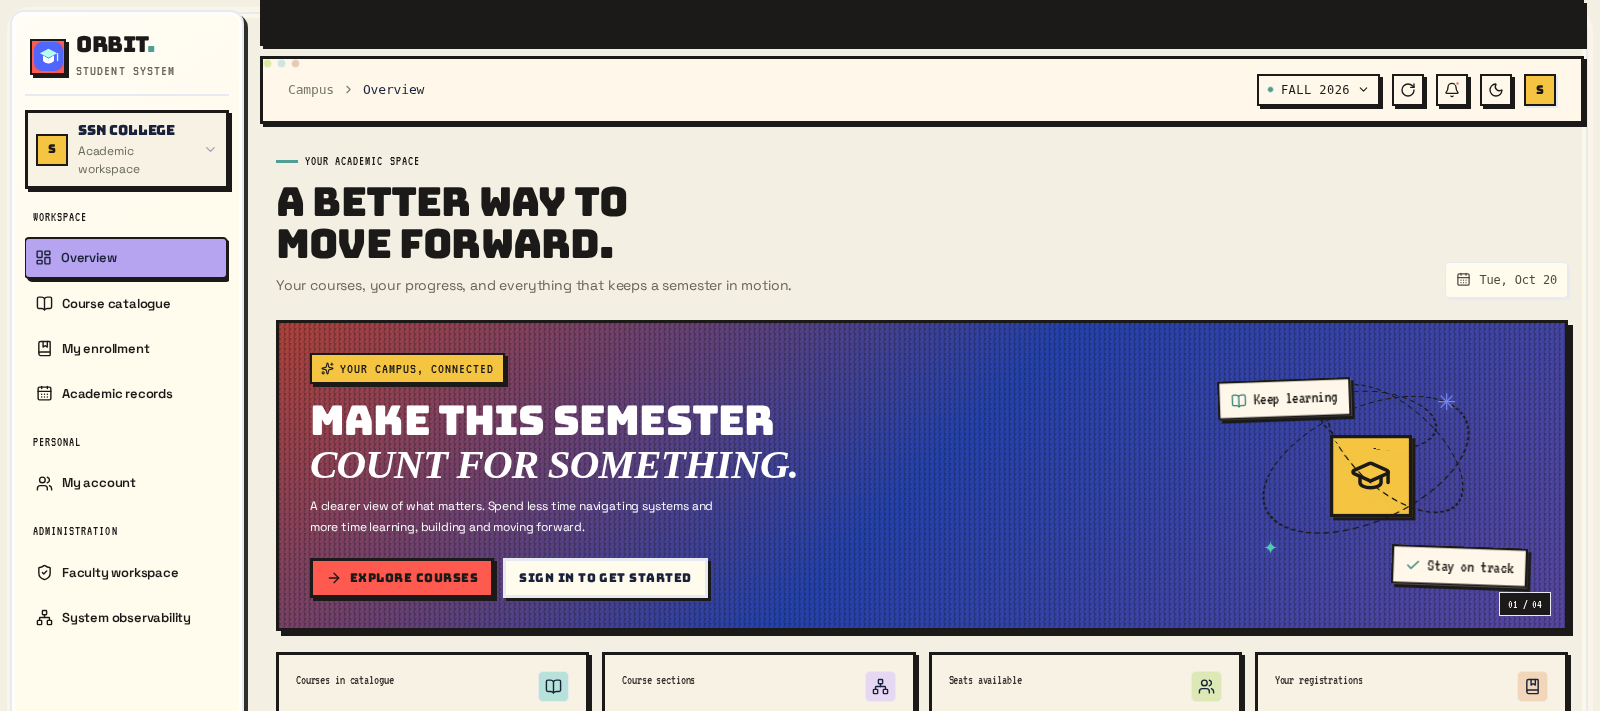
\includegraphics[width=0.62\linewidth]{screenshots/report-cover-crop.png}}
\end{center}
\vspace{3mm}
{\small\color{muted}Student and staff workflows shown in the local application using synthetic demonstration data.}\par
\vspace{4mm}
{\color{teal}\bfseries REPORT DETAILS}\par
\vspace{2mm}
\begin{tabularx}{\linewidth}{@{}>{\color{muted}\bfseries}p{0.28\linewidth}X@{}}
Document & Technical system-design report \\
Review & Design and verification \\
Date & 21 October 2026 \\
Verification environment & Local prototype; synthetic data; PostgreSQL 17.11 \\
\end{tabularx}
\vspace{2mm}
{\color{teal}\bfseries PROJECT TEAM}\par
\vspace{2mm}
\begin{tabularx}{\linewidth}{@{}X X@{}}
Tanish S K & Tarun S \\
{\small\color{muted}3122245001180} & {\small\color{muted}3122245001182} \\
Sujith M & Velamapalli Hemanth Raj Sreyash \\
{\small\color{muted}3122245001172} & {\small\color{muted}3122245001195} \\
\end{tabularx}
\vfill
\rule{\linewidth}{0.6pt}\par
{\small\color{muted}Coursework prototype. Results document tested local behavior; they are not production certification or capacity claims.}
\end{titlepage}
\hypersetup{pageanchor=false}
\pagenumbering{roman}
\chapter*{Abstract}\addcontentsline{toc}{chapter}{Abstract}
Student information systems combine high-contention registration workflows with sensitive academic records. This report presents the design and local verification of Orbit SIS, a full-stack prototype built with React, FastAPI, SQLAlchemy, and PostgreSQL. The principal design decision is to make PostgreSQL the authority for enrollment capacity: a conditional seat-reservation update and the enrollment insert execute in one transaction, with rollback on conflict. In an isolated PostgreSQL 17.11 verification environment, the automated suite reported 23 passing tests; two targeted concurrency tests checked seat-capacity and duplicate-enrollment invariants. Fresh-database migrations, schema-drift checks, Ruff, the frontend production build, five live API smoke checks, and seven desktop UI captures also passed in the recorded run. The report separates these results from historical, single-run Locust measurements and from process-local demonstrations of caching, rate limiting, hash-ring routing, and telemetry. On 21 October, the PostgreSQL suite was rerun after changing the 64-bit ID API to return strings; Postman collection verification passed 24 assertions, and a controlled Apache JMeter read workload completed with zero errors. An unpaced JMeter overload run also demonstrated HTTP 429 admission control. These are local checks, not production-capacity claims. The report documents limitations, reproduction steps, and the next engineering gates. The evidence supports the tested local behaviors; it does not establish production security, availability, or scale.

\textbf{Keywords:} student information system, transactional consistency, PostgreSQL, concurrent enrollment, system design, verification
\clearpage
\tableofcontents
\clearpage
\listoffigures
\clearpage
\listoftables
\clearpage
\hypersetup{pageanchor=true}
\pagenumbering{arabic}

\chapter{Problem and design objectives}
\section{Context}
Registration is a consistency-sensitive workflow. Several students may request the last available seat at nearly the same time. A design that checks capacity in the application and updates it later leaves a race window: two requests may observe the same remaining seat. Academic records also require controlled access, predictable validation, and a clear authoritative data store.

Orbit SIS was developed as a local full-stack prototype for student and staff workflows, with additional system-design experiments that demonstrate caching, rate limiting, ID generation, short links, crawling, routing, and telemetry. The report focuses on what was implemented and what was verified, rather than presenting each experiment as production infrastructure.

\section{Design objectives}
\begin{enumerate}
\item Preserve enrollment invariants under concurrent requests.
\item Keep authentication, authorization, and request validation in the API layer.
\item Keep persistent academic state in PostgreSQL.
\item Make component boundaries and trade-offs explicit.
\item Support reproducible local checks and distinguish fresh results from historical measurements.
\end{enumerate}

\section{Scope and non-goals}
The verification covers a local prototype and synthetic records. It does not certify production security, high availability, disaster recovery, multi-region behavior, or production throughput. Cache, rate limiter, hash ring, and telemetry experiments are process-local. The crawler's public-network behavior was not verified because DNS/network reachability was unavailable in the recorded environment.

\chapter{Architecture and data model}
\section{Runtime architecture}
The React interface presents student and faculty workflows. FastAPI exposes HTTP endpoints and applies validation and access checks. SQLAlchemy connects the API to PostgreSQL, which stores student profiles, courses, offerings, enrollments, and academic records. The database is the source of truth for seat capacity and enrollment state. The transaction and locking model follows PostgreSQL's documented concurrency mechanisms [3, 4].

\begin{figure}[htbp]
\centering
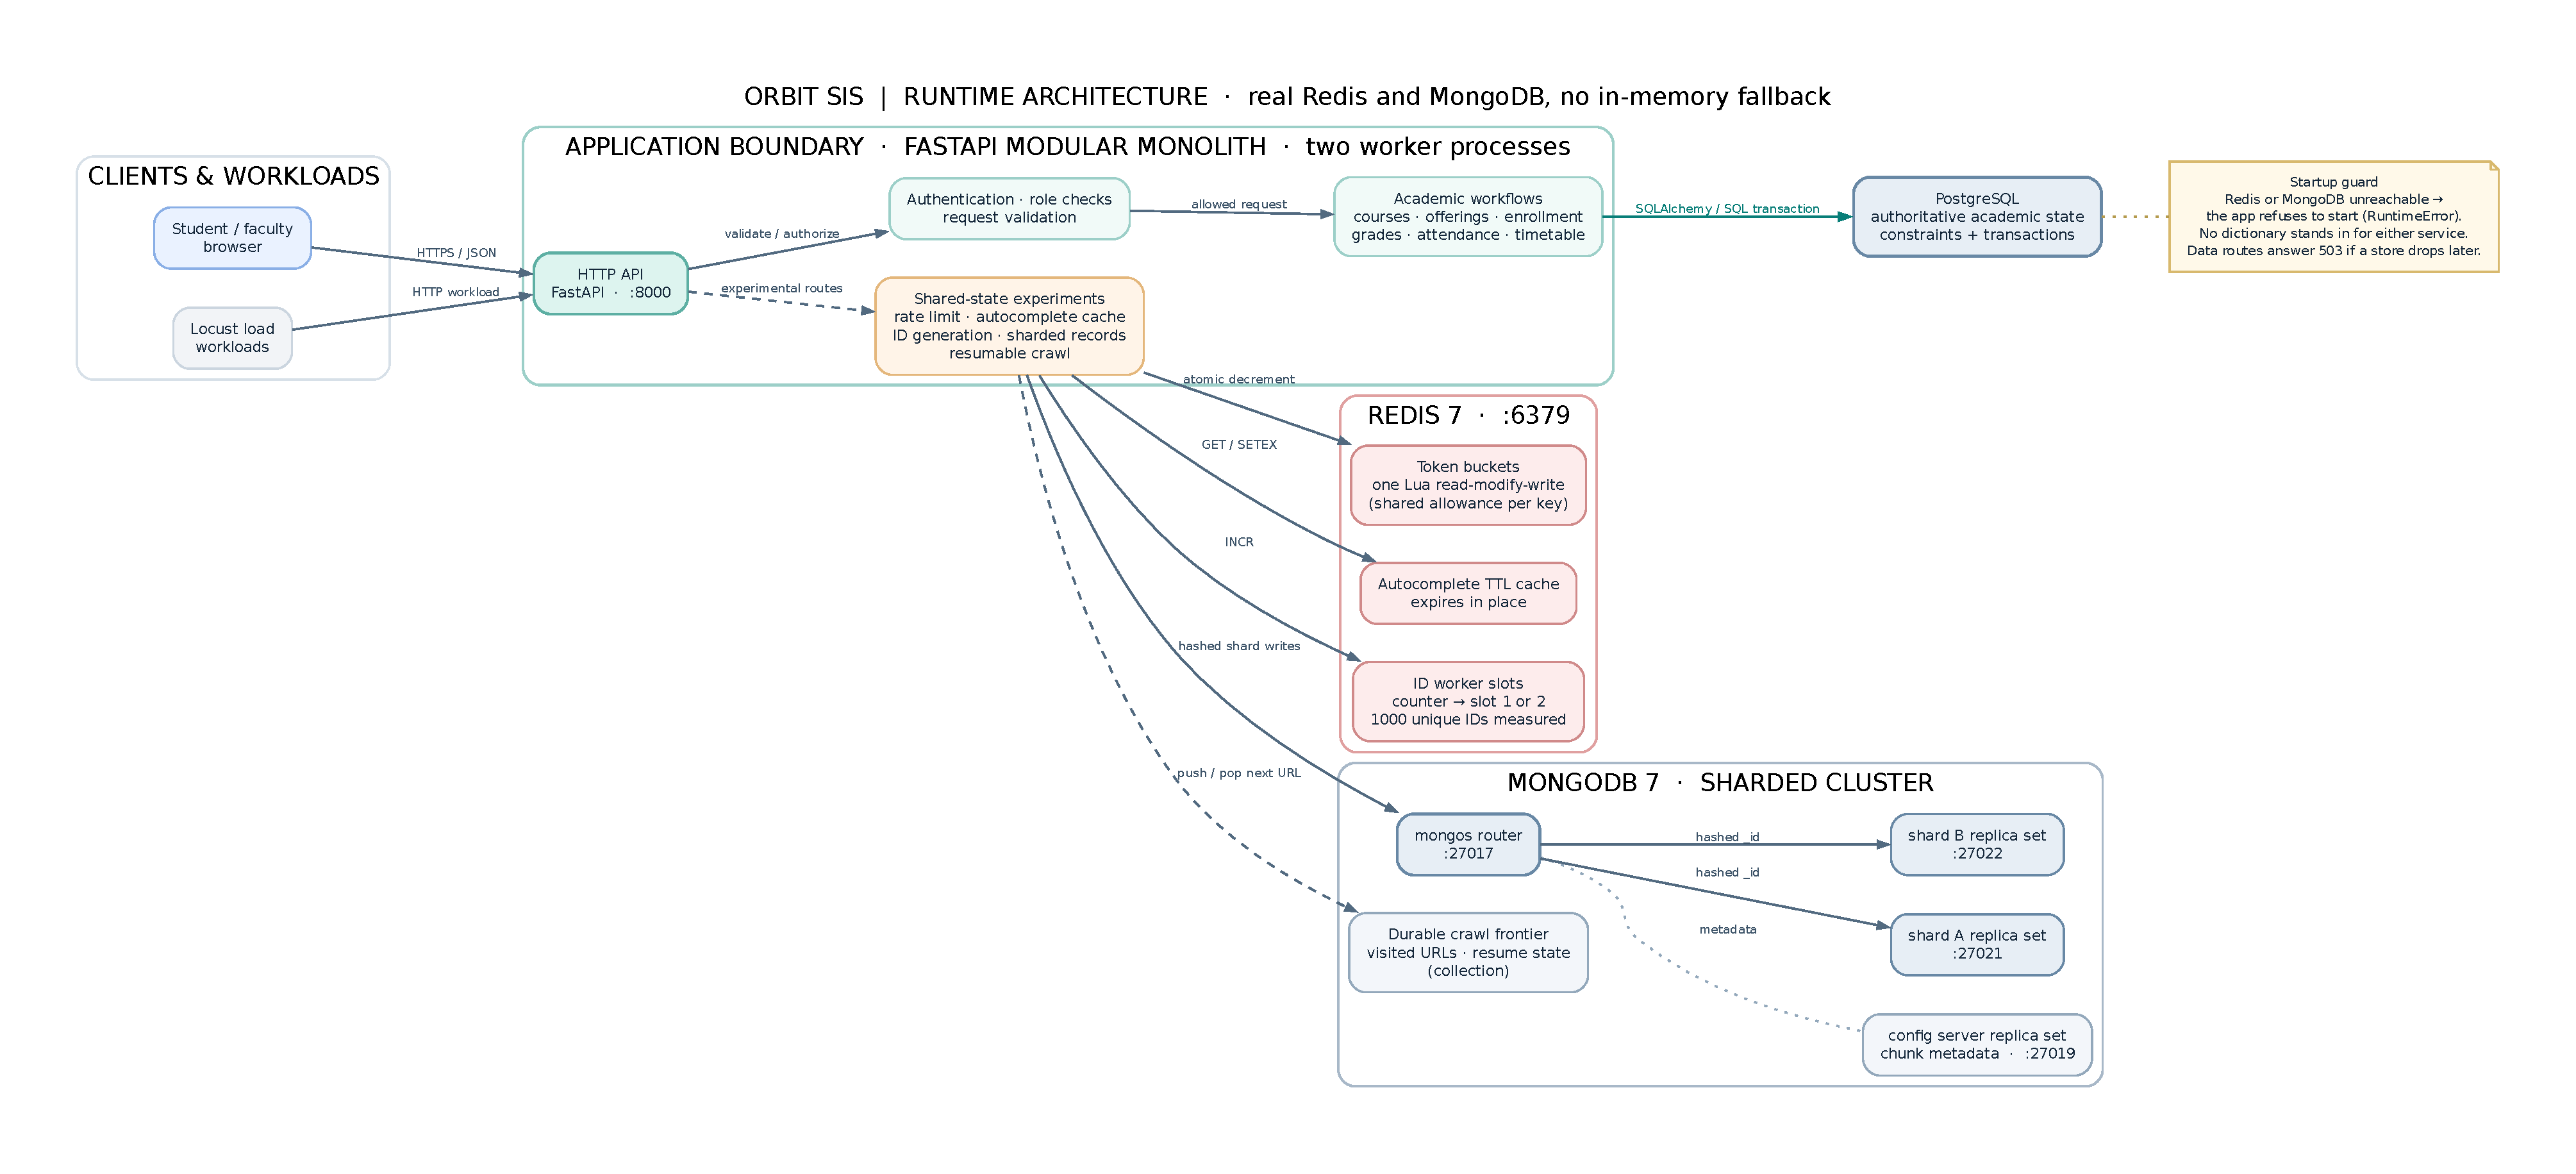
\includegraphics[width=\linewidth]{diagrams/architecture.pdf}
\caption[Runtime architecture]{Runtime architecture and trust boundaries. Solid edges show primary request/data paths; dashed edges indicate experimental or auxiliary paths.}
\label{fig:architecture}
\end{figure}

\section{Core entities}
\begin{table}[htbp]
\centering\small
\caption{Core domain entities and responsibilities}\label{tab:entities}
\begin{tabularx}{\linewidth}{@{}lX@{}}\toprule
\textbf{Entity} & \textbf{Responsibility} \\midrule
Student & Identity, profile, and student-specific access scope. \\
Course & Catalogue metadata shared across offerings. \\
Course offering & Term/section, status, capacity, and enrolled count. \\
Enrollment & Student-to-offering relationship, state, and request/idempotency context. \\
Academic records & Attendance, assessment, grades, timetable, and notifications. \\bottomrule
\end{tabularx}
\end{table}

\section{Consistency boundary}
The cache, rate limiter, hash ring, and telemetry components demonstrate mechanisms in a single process. Their state is not coordinated across API workers. They must not be treated as authoritative for academic state. PostgreSQL constraints and transactional updates protect enrollment; a cache hit or routing decision must never determine whether a seat exists.

\chapter{Transactional enrollment correctness}
\section{Invariant}
For each offering, the primary capacity invariant is
\begin{equation}\label{eq:capacity}
0 \leq \texttt{enrolled\_count} \leq \texttt{capacity}.
\end{equation}
The endpoint performs a conditional update that reserves a seat only while the offering is open and the enrolled count is below capacity. The enrollment insert occurs in the same transaction. If the insert fails because of a uniqueness conflict, the transaction rolls back the counter update.

\section{Request sequence}
\begin{figure}[htbp]
\centering
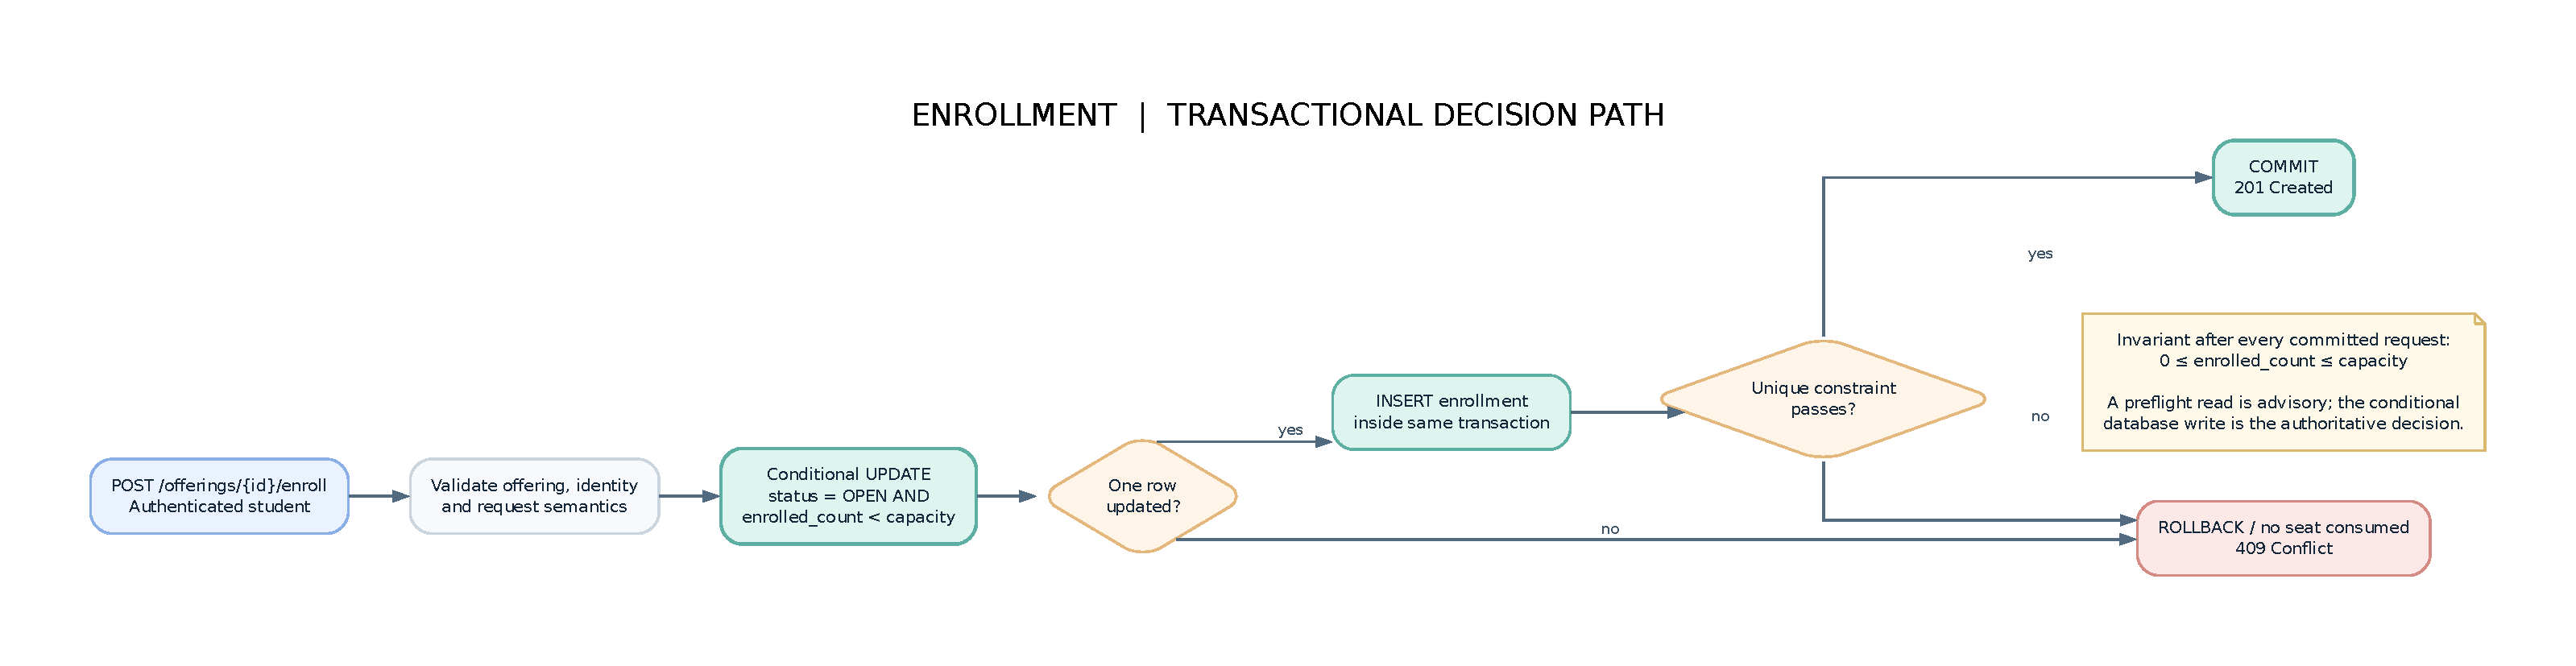
\includegraphics[width=\linewidth]{diagrams/enrollment-transaction.pdf}
\caption[Enrollment transaction path]{Enrollment decision path. A conditional database write decides capacity; the seat update and enrollment insert commit or roll back together.}
\label{fig:transaction}
\end{figure}

\section{Concurrent capacity test}
Twenty distinct students concurrently attempted enrollment into an offering with five seats using 20 worker threads. The test expected five HTTP 201 responses, fifteen HTTP 409 responses, an enrolled count of five, and five active enrollment rows. The recorded PostgreSQL-backed run passed this invariant.
\begin{figure}[htbp]
\centering
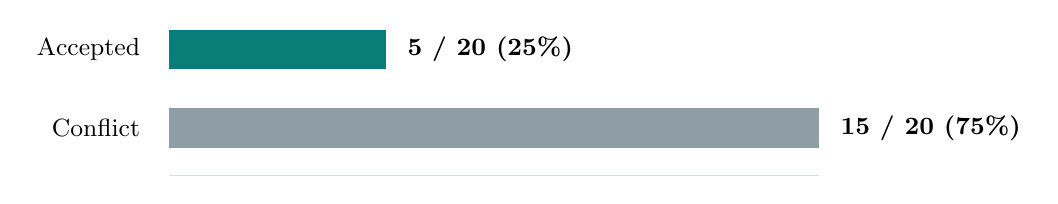
\begin{tikzpicture}[x=1cm,y=1cm]
\node[anchor=east,font=\small] at (0,1.1) {Accepted};
\fill[teal] (0.25,0.85) rectangle (3.0,1.35);\node[anchor=west,font=\small\bfseries] at (3.15,1.1) {5 / 20 (25\%)};
\node[anchor=east,font=\small] at (0,0.1) {Conflict};
\fill[muted!65] (0.25,-0.15) rectangle (8.5,0.35);\node[anchor=west,font=\small\bfseries] at (8.65,0.1) {15 / 20 (75\%)};
\draw[rulegray] (0.25,-0.5) -- (8.5,-0.5);
\end{tikzpicture}
\caption{Expected and observed outcome distribution for the five-seat concurrency test.}
\label{fig:capacity-results}
\end{figure}

\section{Duplicate-request race}
A second test submitted two simultaneous enrollment attempts for the same student and offering with distinct idempotency keys. The test asserts one success, one conflict, one active enrollment, and a single counter increment. This is targeted evidence for the tested race, not proof that every endpoint or every deployment condition is race-free.

\chapter{Implementation and design trade-offs}
\section{Component boundaries}
\begin{table}[htbp]
\centering\small
\caption{Implemented mechanisms and their current boundaries}\label{tab:tradeoffs}
\begin{tabularx}{\linewidth}{@{}p{0.24\linewidth}XX@{}}\toprule
\textbf{Component} & \textbf{Demonstrated behavior} & \textbf{Boundary and next step} \\midrule
PostgreSQL & Persistent academic state, conditional seat reservation, uniqueness constraints. & Add backup/restore drills, connection-pool tuning, and operational monitoring. \\
TTL/LRU cache & Process-local autocomplete reuse. & Not shared across instances; use a shared cache if deployment requires it. \\
Token-bucket limiter & Process-local burst control. & Limits are not coordinated across workers; validate quotas against legitimate traffic. \\
Consistent hash ring & Virtual-node routing experiment. & Does not migrate or replicate data; it is a routing demonstration. \\
Telemetry & In-memory request counts and latency samples. & Resets on restart; production monitoring needs persistent metrics and dashboards. \\
Crawler & Bounded same-host crawler logic. & Public-network behavior was not verified; review SSRF and DNS-pinning risks before external use. \\
ID endpoint & Returns 64-bit identifiers as JSON strings; uniqueness is asserted before serialization. & Clients must treat IDs as opaque strings; a string response avoids JavaScript Number precision loss. \\bottomrule
\end{tabularx}
\end{table}

\section{Security and privacy scope}
The prototype includes role/self-access checks for staff-only academic mutations and student record reads. Staff promotion is a trusted local command-line operation. Token revocation/refresh and production identity controls are not implemented. The application should not be exposed publicly or populated with real student records without additional security, privacy, and operational review. The crawler also requires independent review before use outside coursework.

\chapter{Verification methodology and results}
\section{Environment and isolation}
The recorded verification used a dedicated PostgreSQL 17.11 container on port 55432 with separate databases for synthetic demo data and the automated test suite. This avoided modifying the pre-existing \texttt{sis} database. Three migration revisions were applied to fresh databases. The UI was served from the production frontend build and used synthetic demo records.

\section{Verification matrix}
\begin{table}[htbp]
\centering\small
\caption{Recorded verification results, 20 October 2026}\label{tab:verification}
\begin{tabularx}{\linewidth}{@{}p{0.36\linewidth}p{0.19\linewidth}X@{}}\toprule
\textbf{Check} & \textbf{Result} & \textbf{Scope} \\midrule
Automated test suite & 23 passed & Full suite against isolated PostgreSQL database. \\
Capacity race & Passed & 20 concurrent students compete for five seats. \\
Duplicate enrollment race & Passed & One active enrollment and one counter increment after concurrent duplicate requests. \\
Alembic migrations & Passed & Three revisions applied to fresh databases. \\
Schema drift check & Passed & No new upgrade operations detected. \\
Ruff & Passed & Application, tests, scripts, and migrations. \\
Frontend build & Passed & TypeScript and Vite production build. \\
Live API smoke checks & 5 / 5 & Health, OpenAPI, course list, autocomplete, and ID endpoint returned HTTP 200. \\
Desktop UI capture & 7 sections & Overview, catalogue, enrollment, records, account, faculty, and observability. \\
Browser JavaScript errors & 0 observed & During the recorded navigation/capture run only. \\
\bottomrule\end{tabularx}
\end{table}

The automated suite emitted an upstream Starlette/httpx test-client deprecation warning. It did not fail the suite, but the dependency stack should be reviewed during maintenance. The public crawler was not verified because DNS/network reachability was unavailable.

\section{Interface evidence}
\begin{figure}[p]
\centering
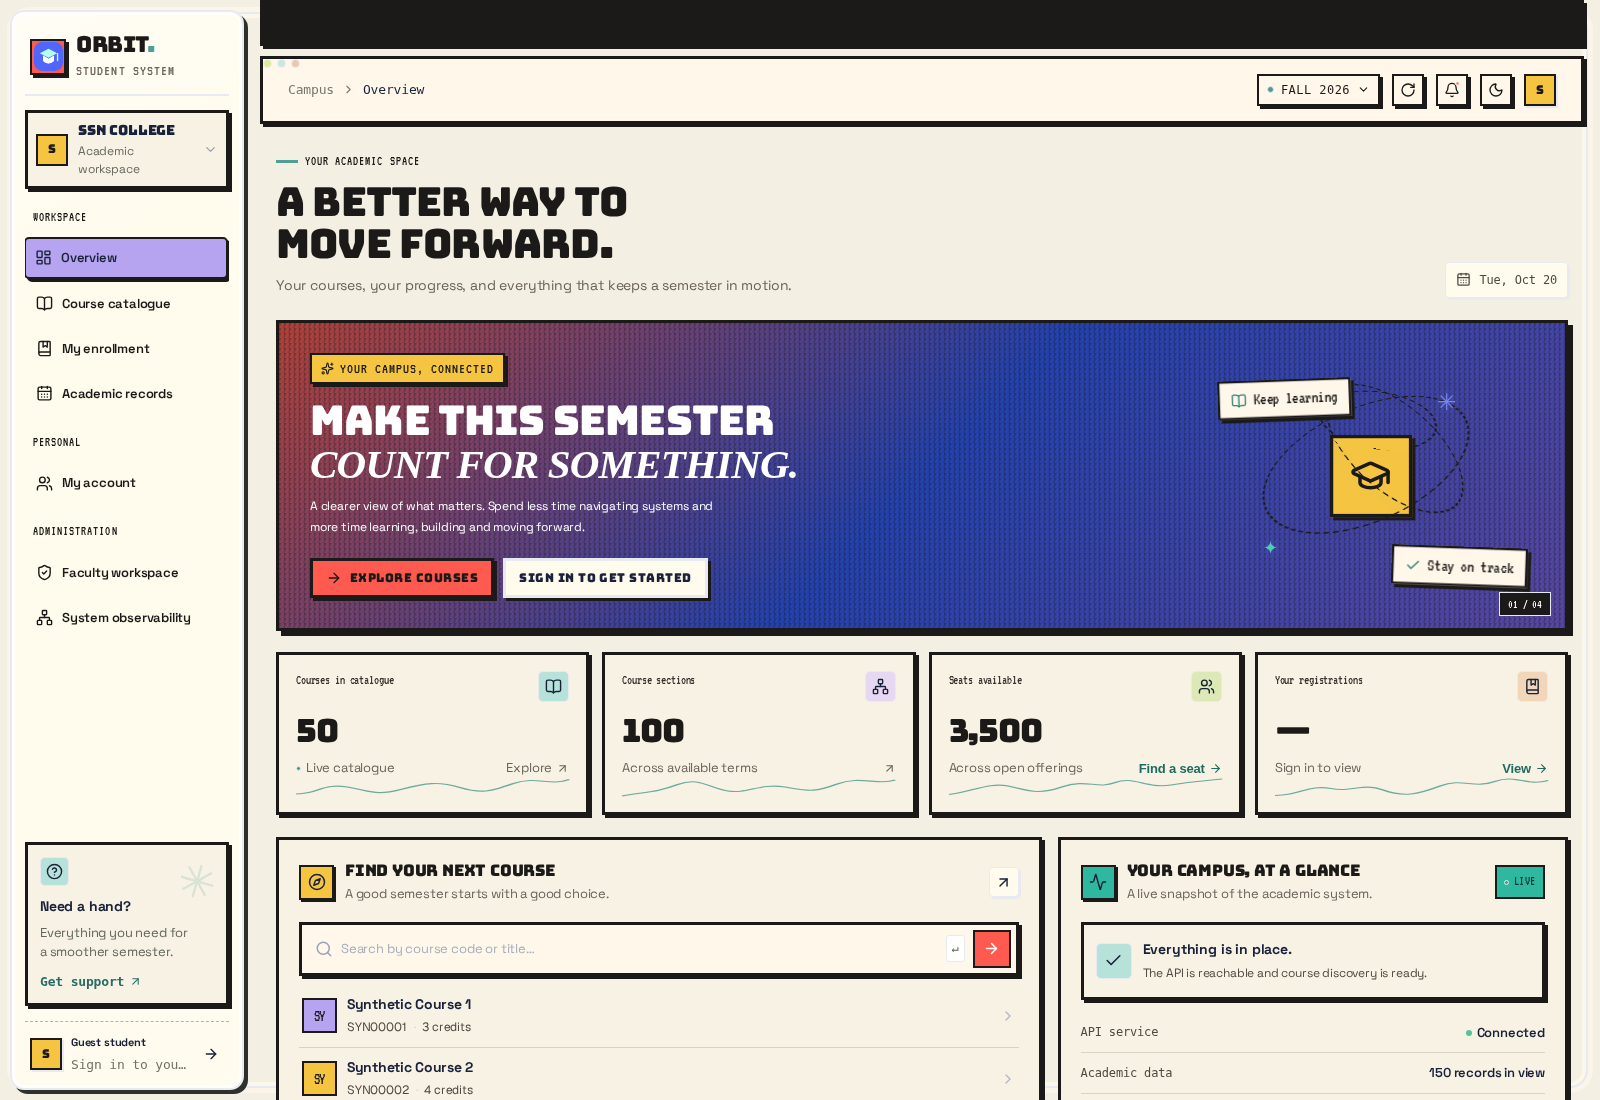
\includegraphics[width=0.98\linewidth,height=0.60\textheight,keepaspectratio]{screenshots/00-overview-viewport.png}
\caption[Dashboard overview]{Dashboard overview captured from the production frontend with synthetic verification data.}
\label{fig:dashboard}
\end{figure}
\begin{figure}[p]
\centering
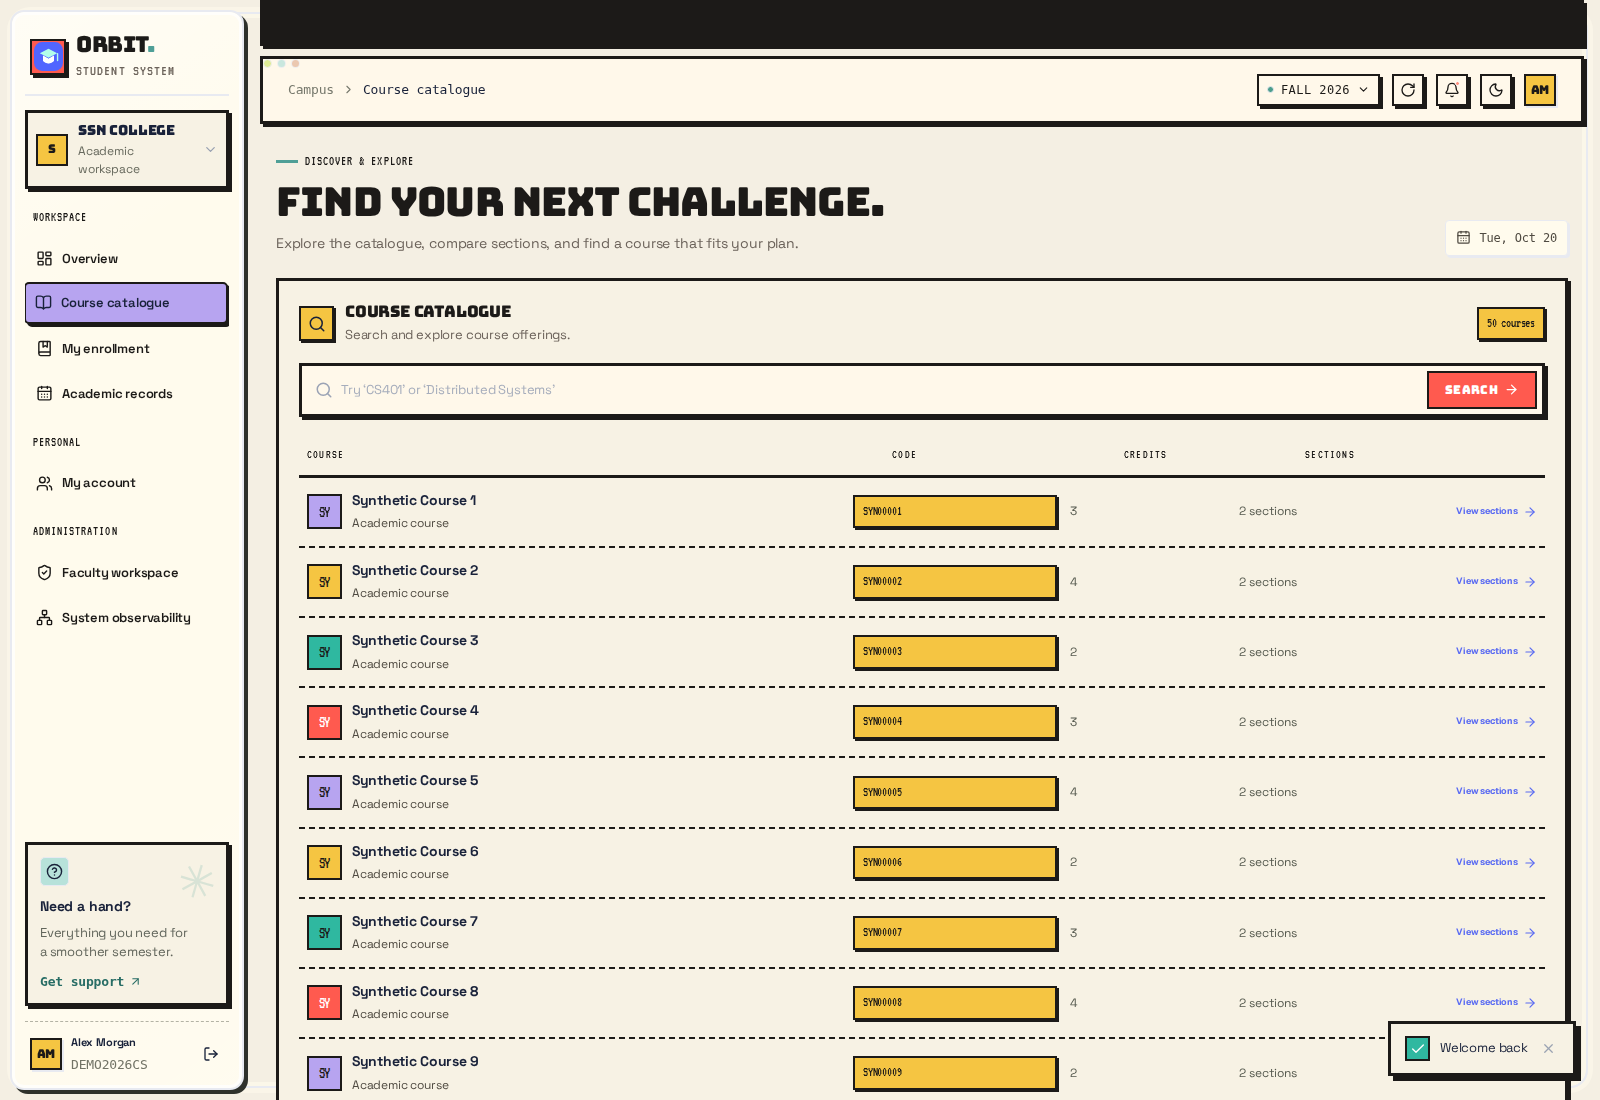
\includegraphics[width=0.98\linewidth,height=0.60\textheight,keepaspectratio]{screenshots/02-courses-desktop.png}
\caption[Course catalogue]{Course catalogue and offering discovery workflow.}
\label{fig:catalogue}
\end{figure}
\begin{figure}[p]
\centering
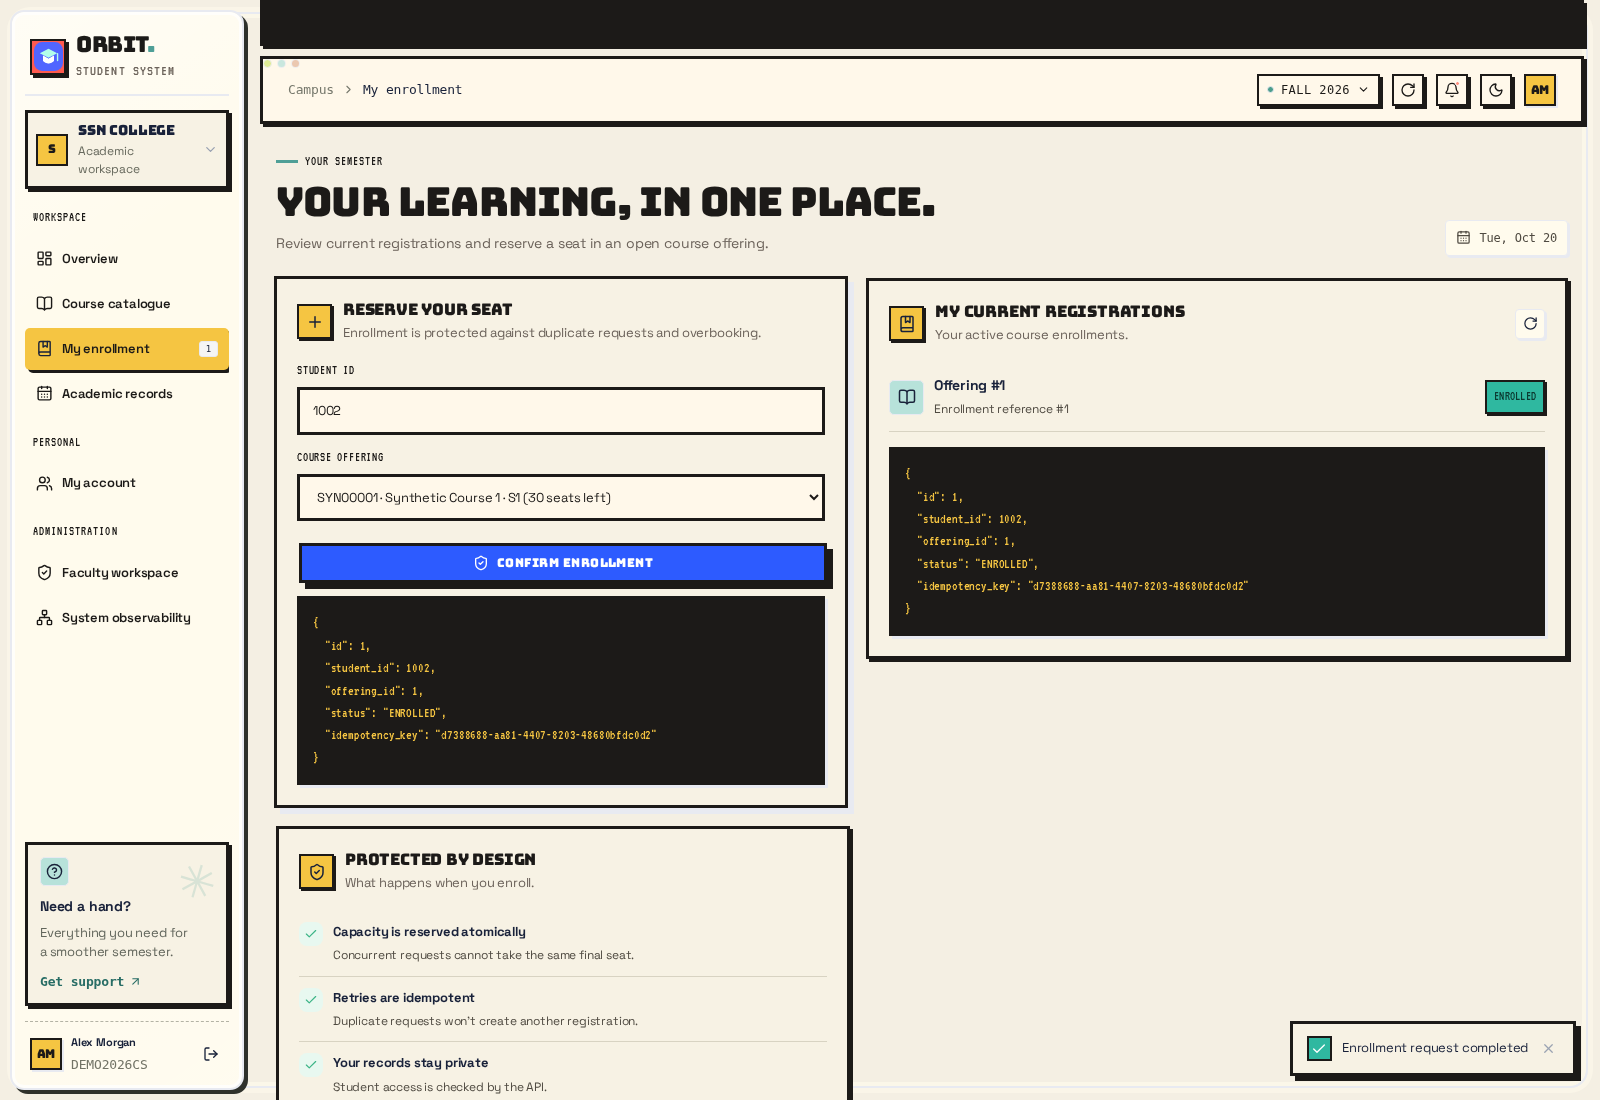
\includegraphics[width=0.98\linewidth,height=0.60\textheight,keepaspectratio]{screenshots/03-enrollment-confirmed.png}
\caption[Successful enrollment]{Successful synthetic student enrollment. The displayed record is demonstration data.}
\label{fig:enrollment-ui}
\end{figure}
\begin{figure}[p]
\centering
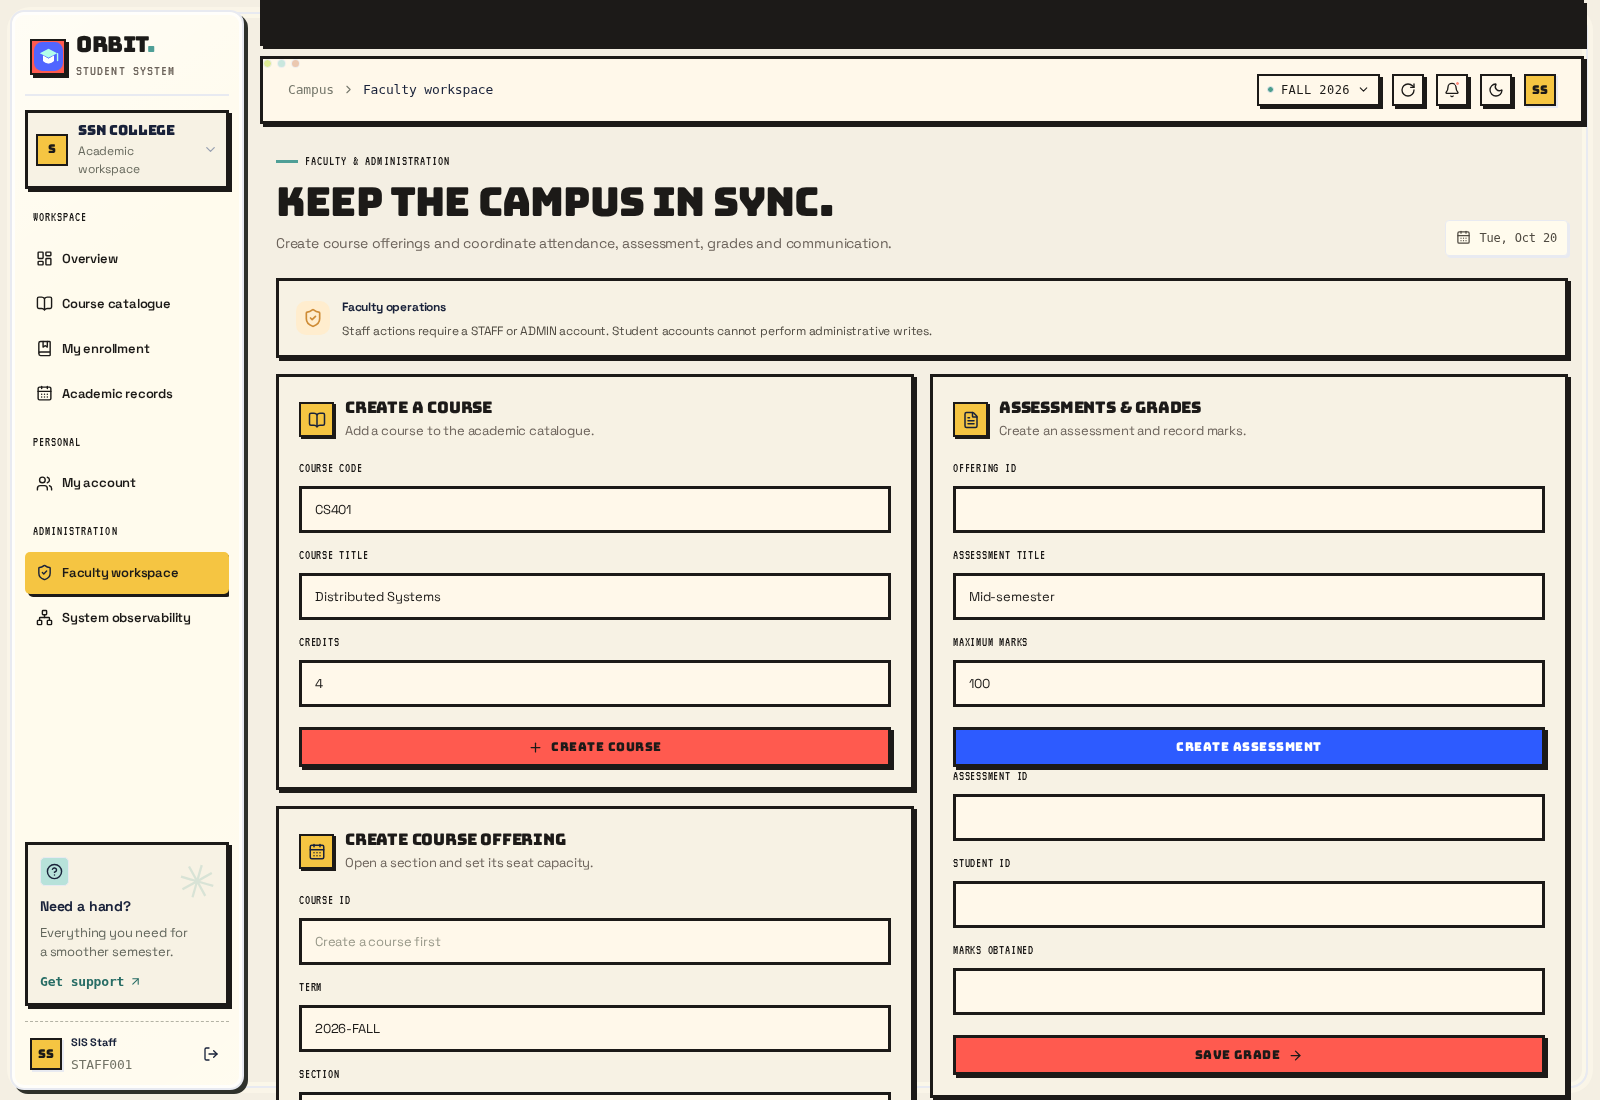
\includegraphics[width=0.98\linewidth,height=0.60\textheight,keepaspectratio]{screenshots/07-faculty-workspace.png}
\caption[Faculty workspace]{Faculty workspace captured after staff sign-in.}
\label{fig:faculty}
\end{figure}
\begin{figure}[p]
\centering
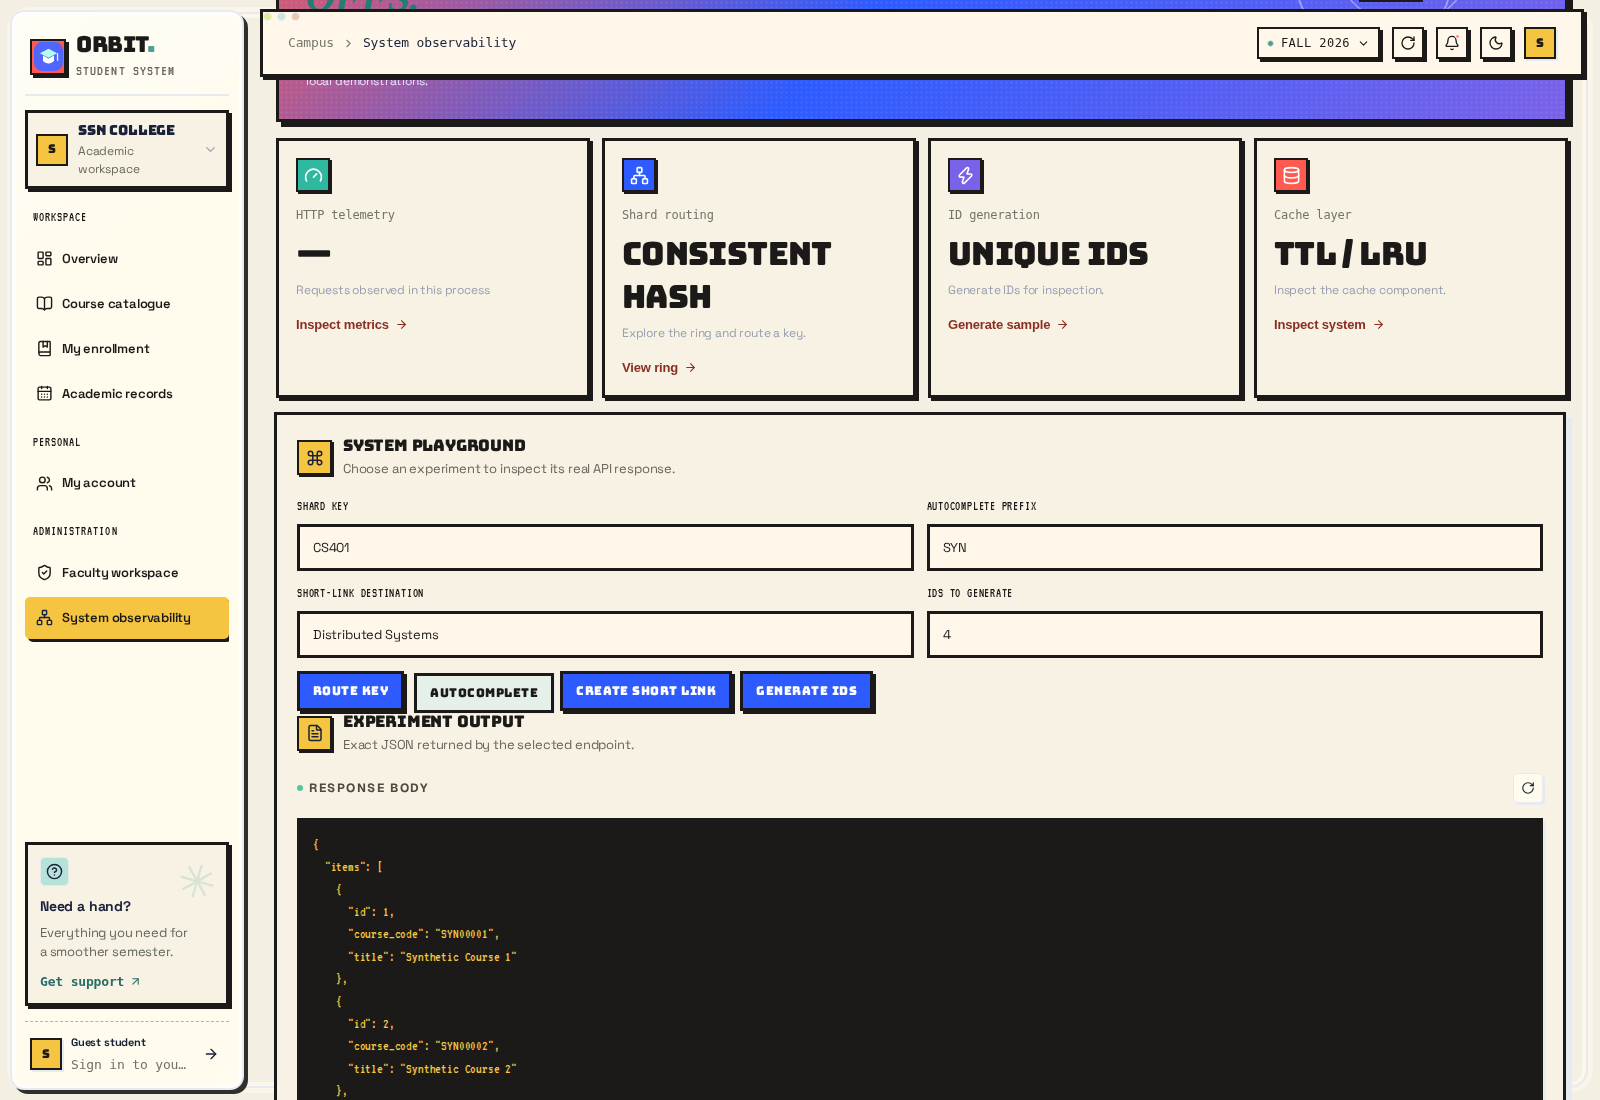
\includegraphics[width=0.98\linewidth,height=0.60\textheight,keepaspectratio]{screenshots/06-system-observability.png}
\caption[System observability]{System observability workspace showing local component experiments.}
\label{fig:observability}
\end{figure}

\chapter{Data integrity and domain model}
\section{Separate catalogue identity from a term-specific offering}
A course and an offering represent different concepts. A course describes reusable catalogue metadata (for example, a course code and title). An offering is a particular instance in a term or section with a status and a finite capacity. Enrollments should reference the offering, not merely the course, because students enroll in a scheduled instance. This distinction permits the same course to run in multiple terms without conflating seat counts or enrollment rosters.

\section{Integrity rules and enforcement layers}
The API validates request shape and access scope; PostgreSQL must enforce invariants that must survive concurrent requests and alternate call paths. Application validation improves error messages but cannot replace a database constraint. The key invariant for an offering is
\begin{equation}
0 \leq enrolled\\_count \leq capacity.
\end{equation}
A unique student/offering relationship prevents duplicate active enrollment rows. The conditional update narrows the capacity decision to one database operation. The insert and counter update share a transaction so a uniqueness failure cannot leave the counter incremented without a matching enrollment.

\begin{table}[htbp]
\centering\small
\caption{Integrity concern, enforcement point, and failure prevented}\label{tab:integrity}
\begin{tabularx}{\linewidth}{@{}p{0.25\linewidth}p{0.29\linewidth}X@{}}\toprule
\textbf{Concern} & \textbf{Enforcement} & \textbf{Failure prevented} \\\midrule
Offering capacity & Conditional update in the transaction & Two concurrent requests consuming the same final seat. \\
Duplicate enrollment & Unique database constraint plus transaction rollback & Multiple active rows for the same student/offering. \\
Role and ownership & API authorization checks & Student reading or modifying another student's restricted records. \\
Schema evolution & Versioned Alembic migrations and fresh-database check & A new installation differing silently from the intended schema. \\
\bottomrule
\end{tabularx}
\end{table}

\section{Idempotency is not the same as uniqueness}
A uniqueness constraint protects stored state, while an idempotency key helps a client safely retry a request after a timeout or lost response. These solve related but different problems. A retry may arrive after the first transaction committed even though the client did not receive the response. A production implementation should persist the key, scope it to the caller and operation, define key retention, and return the original result for a repeated request. The recorded duplicate-race test verifies the implemented endpoint's stated behavior; it does not establish a complete cross-endpoint idempotency protocol.

\chapter{Architecture decisions and alternatives}
\section{Decision: a modular API with one authoritative relational store}
For a coursework system with tightly related academic records, a modular monolith keeps enrollment, authorization, and database transaction boundaries in one deployable service. This avoids introducing network failure modes between separate services before the domain boundaries or operational needs justify them. PostgreSQL provides durable relational state, constraints, and transactions for relationships that must remain consistent.

\section{Rejected or deferred alternatives}
\begin{table}[htbp]
\centering\small
\caption{Architecture alternatives and reasons for deferral}\label{tab:alternatives}
\begin{tabularx}{\linewidth}{@{}p{0.25\linewidth}p{0.32\linewidth}X@{}}\toprule
\textbf{Alternative} & \textbf{Potential benefit} & \textbf{Reason deferred / trigger to revisit} \\\midrule
Microservices for each academic domain & Independent deployment and scaling & Adds service discovery, network failures, distributed tracing, and cross-service consistency. Revisit only with clear ownership and independent scaling needs. \\
Cache as authority for seats & Low-latency reads & Cache state can be stale and does not provide the required transactional invariant. Keep the database authoritative. \\
Application-only capacity check & Simple endpoint code & Check-then-write races under concurrent requests. Use a conditional write and transaction. \\
Distributed cache and rate-limit service & Shared state across API workers & Useful for multi-instance deployment, but current experiments are process-local. Add only with explicit deployment requirements and integration tests. \\
Database sharding now & Potential horizontal data distribution & The project has no measured database bottleneck or implemented migration/replication path. Hash-ring routing alone is not sharding. \\
\bottomrule
\end{tabularx}
\end{table}

\section{Why the consistency boundary matters}
The primary failure to prevent is not a slow response; it is a false academic state, such as two students being assigned one seat or a counter claiming a seat is occupied when no enrollment exists. The design therefore prioritizes transactional correctness over using an eventually consistent cache for enrollment writes. Read optimization can be introduced around that boundary only if invalidation and stale-read behavior are explicitly defined.

\section{Operational boundaries of auxiliary components}
The TTL/LRU cache, token-bucket limiter, hash-ring router, and telemetry collector are in-process experiments. A process restart clears their state, and separate workers may maintain different views. The hash ring demonstrates key-to-node assignment; it does not move database rows, replicate data, rebalance storage, or recover failed nodes. The crawler is additionally an outbound-network boundary and must be reviewed for private-address access, DNS rebinding, redirects, request budgets, and response-size limits before external use.

\chapter{Test strategy, reproducibility, and evidence quality}
\section{Layered verification strategy}
The checks are deliberately layered because no single green command proves overall correctness:
\begin{enumerate}
\item \textbf{Static checks:} Ruff catches selected Python style and correctness issues; the frontend production build checks TypeScript and bundling. Neither executes all runtime paths.
\item \textbf{Database migration checks:} applying all revisions to a fresh database tests bootstrap reproducibility; a schema-drift check tests whether the current models imply unrecorded migration operations.
\item \textbf{Automated tests:} the recorded suite exercises API and domain assertions against PostgreSQL rather than relying only on an in-memory substitute.
\item \textbf{Targeted concurrency tests:} simultaneous requests test the two named enrollment races and assert both response outcomes and final stored state.
\item \textbf{Smoke checks:} live endpoints verify a small set of routes can respond; this is not broad endpoint coverage.
\item \textbf{Browser checks:} navigation and screenshots confirm the tested UI paths rendered without observed JavaScript errors in that run. They do not prove accessibility or all-device compatibility.
\item \textbf{Load experiments:} Locust observations characterize a short offered workload and should be repeated with controlled conditions before drawing capacity conclusions.
\end{enumerate}

\section{Isolation and repeatability}
The recorded run used a dedicated PostgreSQL 17.11 container and separate databases for synthetic demonstration data and the test suite, on port 55432. This separation was intentional: the existing local database was not the target of the final verification. A repeatable test record should include the commit or source snapshot, dependency lock state, database version, migration revision, test command, environment flags, seed-data procedure, and raw logs. The values in this report describe the recorded run and should not be assumed to describe a later code snapshot unless the checks are repeated.

\section{What the evidence does and does not establish}
\begin{table}[htbp]
\centering\small
\caption{Evidence strength and limits}\label{tab:evidence-strength}
\begin{tabularx}{\linewidth}{@{}p{0.28\linewidth}p{0.33\linewidth}X@{}}\toprule
\textbf{Evidence} & \textbf{Supports} & \textbf{Does not establish} \\\midrule
23 passing automated tests & Assertions in the recorded test suite pass on the configured PostgreSQL database. & Absence of untested defects, security vulnerabilities, or all possible race conditions. \\
20-request/five-seat race & Capacity invariant held for the tested concurrent workload. & Behavior under arbitrary load, multiple regions, or database failover. \\
Fresh migrations and schema check & Schema can be created from the recorded migration history without detected drift. & Disaster recovery, rollback safety for every future migration, or production data migration. \\
Five live smoke checks & Five named endpoints returned HTTP 200. & Correct authorization for every route or complete API health. \\
Single-run Locust sample & Observed latency and errors for one short local workload. & Stable throughput, capacity ceiling, statistical confidence, or production SLOs. \\
Browser screenshots and no observed JS errors & Selected pages rendered during the capture session. & Accessibility conformance, cross-browser correctness, or complete user acceptance. \\
\bottomrule
\end{tabularx}
\end{table}

\section{Benchmark interpretation}
The reported request rate is a property of a specific test setup, request mix, duration, local machine, and database state. It is not a capacity limit. The 20-second Locust window is short enough that startup, connection warm-up, cache state, and test scheduling can materially affect results. The cache-enabled and cache-disabled autocomplete runs also have different total request counts, so their latency difference is a useful hypothesis rather than a controlled causal estimate. The observed 35.95\\% HTTP 429 fraction under the limiter workload should be interpreted together with legitimate-request latency and the intended quota policy.

A stronger follow-up benchmark should record hardware and OS, exact code revision, database configuration and dataset size, warm-up period, steady-state duration, user arrival pattern, per-endpoint request mix, errors/timeouts, and CPU/memory for API, database, and load generator. Repeat at least several runs per configuration; report median and spread rather than only one point estimate. Test realistic and overload scenarios separately, and do not tune a limiter solely to maximize requests per second.

\chapter{Security, privacy, and release readiness}
\section{Current safeguards and residual risks}
The prototype includes role/self-access checks for selected operations and uses synthetic data in the recorded evidence. Staff promotion is a trusted local command-line action. Token refresh/revocation and production identity integration are not implemented. A local demonstration should not be exposed to the public internet or populated with real student records on the strength of the current tests.

The crawler deserves separate threat analysis because a user-controlled URL can make the server initiate network requests. Before enabling it in a reachable deployment, enforce an allowlist or strict public-address policy, resolve and validate addresses at connection time, re-check redirects, reject loopback/private/link-local/reserved IP ranges, cap response size and time, and log/limit requests. DNS validation alone can be insufficient if the resolved address changes between validation and connection.

\section{Release gates}
\begin{table}[htbp]
\centering\small
\caption{Minimum next gates before a non-local deployment}\label{tab:release-gates}
\begin{tabularx}{\linewidth}{@{}p{0.24\linewidth}p{0.51\linewidth}X@{}}\toprule
\textbf{Gate} & \textbf{Required work} & \textbf{Evidence to retain} \\\midrule
Identity and authorization & Production identity integration, token lifecycle, role policy review, negative authorization tests. & Threat model and automated allow/deny matrix. \\
Data protection & Secrets management, TLS termination, retention policy, backups, restore drills, audit of sensitive access. & Configuration review and successful restore record. \\
Distributed operation & Shared limiter/cache where required, connection pool limits, health checks, graceful shutdown. & Multi-worker integration tests and failure tests. \\
Performance and reliability & Repeated load tests, saturation tests, DB connection/lock observations, explicit SLO targets. & Reproducible benchmark report with raw results. \\
Outbound crawler & SSRF/DNS-pinning controls and network-enabled security tests. & Test matrix covering private IPs, redirects, DNS changes, and size/time limits. \\
Browser correctness & Accessibility audit, cross-browser and responsive regression. & Automated accessibility findings and viewport/browser matrix. \\
\bottomrule
\end{tabularx}
\end{table}

\chapter[Performance observations]{Performance observations\\and limitations}
\section{Postman and Apache JMeter verification — 21 October 2026}
Postman Desktop 12.33.2 was installed, and the exported collection was executed with Newman 6.2.3; Apache JMeter 5.6.3 was used for the controlled and overload runs. The API ran locally at \texttt{127.0.0.1:8000} against the existing development database and synthetic records. The Postman collection creates one uniquely named synthetic student account; no real student data were used. The retained machine-readable run summary has response bodies and bearer tokens redacted.

\begin{table}[htbp]
\centering\small
\caption{Tool-assisted API verification, 21 October 2026}\label{tab:tool-verification}
\begin{tabularx}{\linewidth}{@{}p{0.29\linewidth}p{0.22\linewidth}X@{}}\toprule
\textbf{Tool / scenario} & \textbf{Observed result} & \textbf{Interpretation} \\\midrule
Postman collection via Newman (fresh rerun) & 13 requests; 24/24 assertions passed; average 20 ms & Checked health, course/offering reads, autocomplete/cache state, 25 unique IDs, ring/metrics metadata, missing authentication, registration/login, student role denial, and invalid credentials. \\
Apache JMeter controlled read workload (fresh rerun) & 10 threads; 2 s ramp; 20 s duration; 185 samples; 0 errors; mean 4.95 ms; median 4 ms; p95 10 ms; 9.84 req/s & A paced local read-only baseline across seven endpoints. This is one short run on a shared laptop, not a production capacity estimate. \\
Apache JMeter unpaced overload experiment (fresh rerun) & 48,459 samples; 40,372 HTTP 429; 8,081 HTTP 200; 6 socket timeouts & Deliberately unpaced traffic; 83.32\% of samples failed, mostly expected HTTP 429 admission-control responses. Six transport timeouts also occurred, so this is not a clean all-429 result or a baseline. \\
Resource-sampled paced repeat & 185 samples; 0 errors; mean 7.37 ms; p95 20 ms; 9.87 req/s & Separate run sampled with pidstat and podman stats: API CPU mean 2.65\%, peak 5.0\%, RSS 14--30 MiB; PostgreSQL container memory 11--22 MB. Not host-wide telemetry. \\
PostgreSQL automated suite & 23 passed & Rerun against a dedicated PostgreSQL test database after the ID serialization fix, including both concurrent enrollment invariants. \\
Ruff static checks & Passed & Application, tests, scripts, and migrations. \\
\bottomrule\end{tabularx}
\end{table}

\begin{figure}[p]
\centering
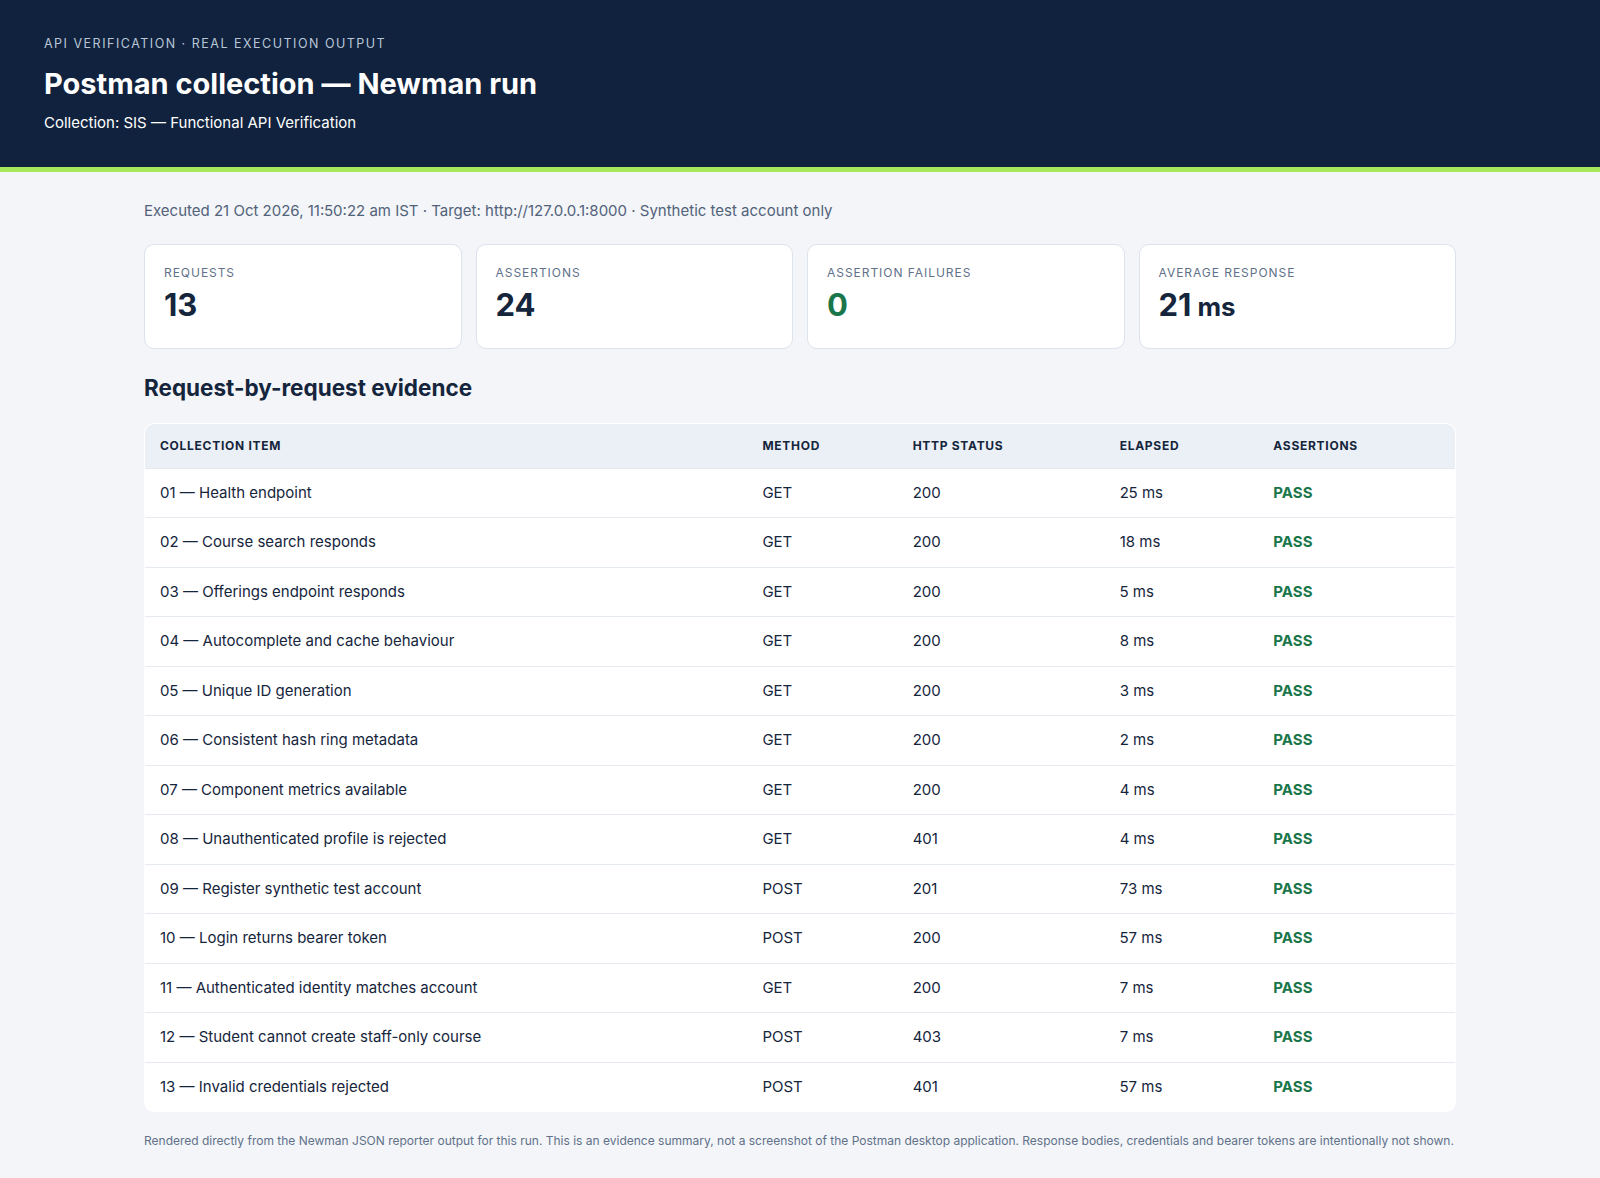
\includegraphics[width=\linewidth,height=0.72\textheight,keepaspectratio]{screenshots/tool-verification/rerun-20261021/postman-newman-run.png}
\caption[Postman collection results]{Evidence summary rendered from the fresh Newman JSON output for the Postman collection. Expected 401 and 403 responses pass their negative-security assertions; this image is not the Postman desktop UI.}
\label{fig:postman-verification}
\end{figure}

\begin{figure}[p]
\centering
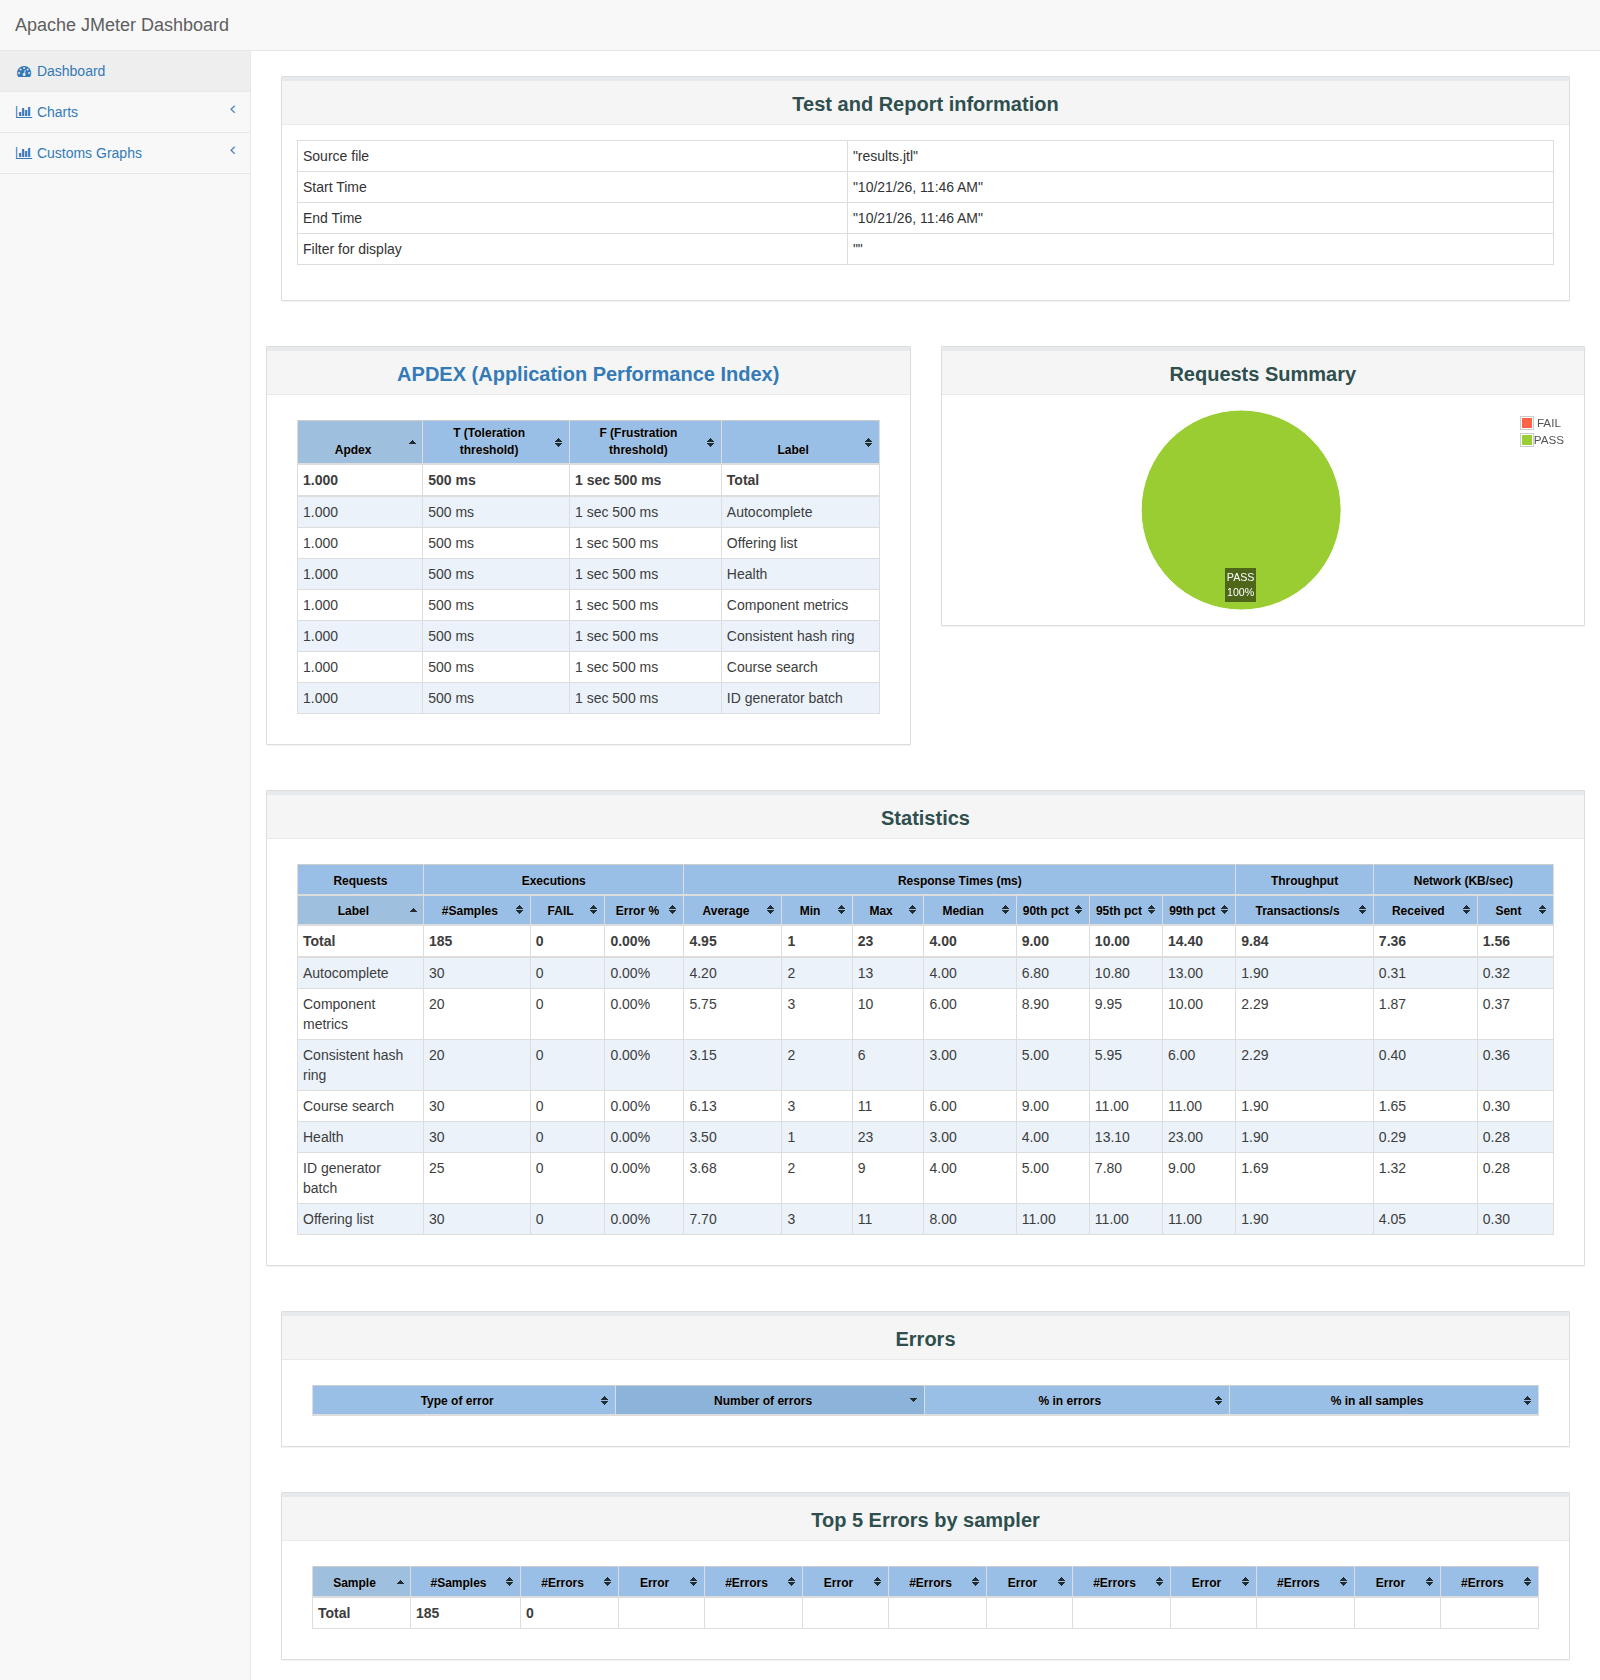
\includegraphics[width=\linewidth,height=0.72\textheight,keepaspectratio]{screenshots/tool-verification/rerun-20261021/jmeter-baseline-dashboard.png}
\caption[Apache JMeter controlled baseline]{Apache JMeter HTML dashboard for the paced read-only baseline: 185 samples and zero failed requests.}
\label{fig:jmeter-baseline}
\end{figure}

\begin{figure}[p]
\centering
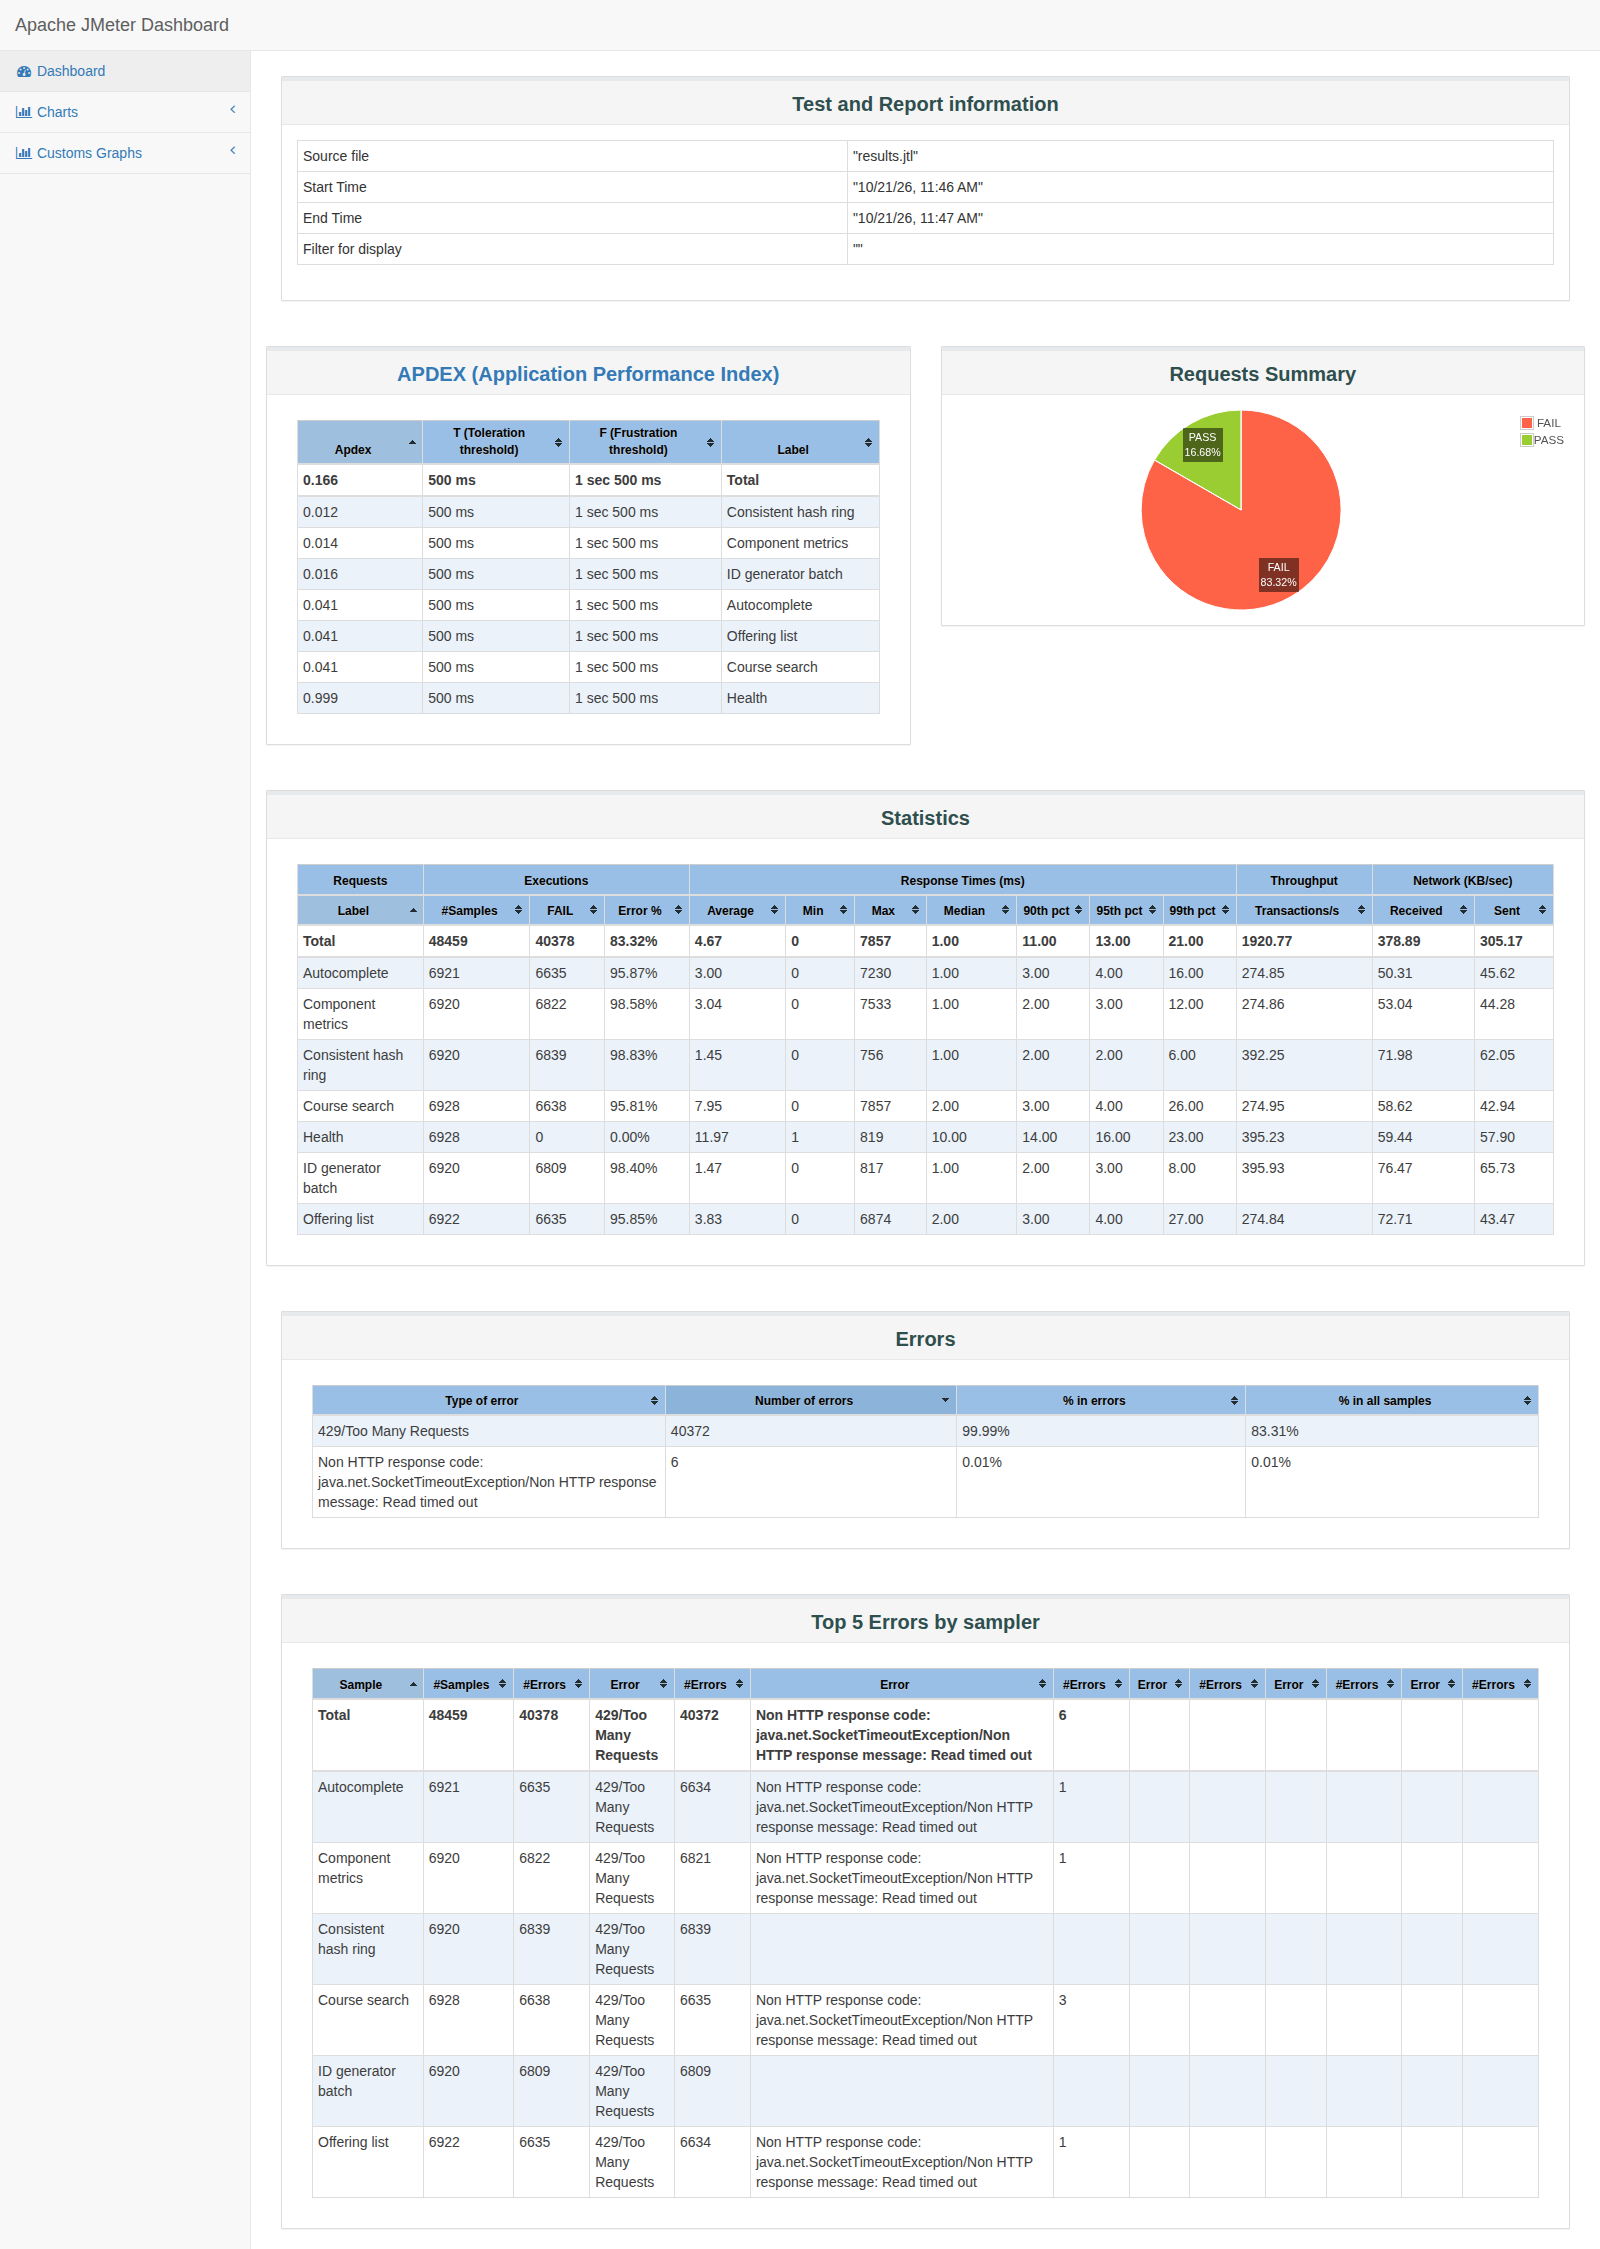
\includegraphics[width=\linewidth,height=0.72\textheight,keepaspectratio]{screenshots/tool-verification/rerun-20261021/jmeter-overload-dashboard.png}
\caption[Apache JMeter overload behavior]{Unpaced overload produced HTTP 429 responses from the token-bucket limiter. The fresh rerun had 83.32\% failed samples, including six socket timeouts as well as expected HTTP 429 responses. This overload result must not be combined with baseline results.}
\label{fig:jmeter-overload}
\end{figure}

The JMeter plan is read-only and does not prove database transaction correctness; the PostgreSQL concurrency tests establish the specific enrollment invariants. The rate limiter and telemetry are process-local, so behavior under multiple workers is not represented. The first ID uniqueness assertion exposed JavaScript precision loss when 64-bit IDs were emitted as JSON numbers. The API now emits IDs as strings and the regression test asserts the string contract. This fixes the API representation issue but does not turn the local ID generator into a distributed, multi-worker generator.

\section{Historical local measurements}
The 19 October Locust runs used 10 users, a spawn rate of two users per second, and a 20-second limit. These are single-run local observations, not fresh measurements from the 20 October verification and not production capacity claims.
\begin{table}[htbp]
\centering\small
\caption{Historical single-run Locust observations (19 October 2026)}\label{tab:locust}
\begin{tabularx}{\linewidth}{@{}Xrrrr@{}}\toprule
\textbf{Workload} & \textbf{Requests} & \textbf{req/s} & \textbf{p95 ms} & \textbf{Failures} \\midrule
Course search/list/offering mix & 681 & 35.82 & 10 & 0 \\
Authenticated profile and academic reads & 669 & 35.27 & 12 & 0 \\
Student account registration writes & 370 & 19.47 & 83 & 0 \\
Autocomplete, cache enabled & 675 & 35.55 & 5 & 0 \\
Autocomplete, cache disabled & 659 & 34.68 & 10 & 0 \\
Course-search overload, limiter enabled & 676 & 35.61 & 10 & 243 HTTP 429 \\
\bottomrule\end{tabularx}
\end{table}

The cache-enabled autocomplete run reported mean latency of 2.88 ms versus 5.85 ms without caching, roughly 50.8\% lower in this run. Median latency fell from 5 ms to 2 ms and p95 from 10 ms to 5 ms. This is a short, single-run observation. Repeated runs with controlled conditions are required before generalizing the effect.

The overload run returned 243 HTTP 429 responses out of 676 requests (35.95\%). This demonstrates admission control under the tested offered load, but also indicates that the quota needs tuning against legitimate traffic and service latency. A separate sample observed approximately 7.4\% average CPU of one logical CPU and 90,660 KiB RSS for the API process; this was not total host or database utilization.

\section{Limitations}
\begin{itemize}
\item No production deployment, availability, security, or capacity certification was performed.
\item Cache, rate limiter, and telemetry state are process-local, not coordinated across workers.
\item The hash-ring experiment does not implement data migration, replication, or failover.
\item The public crawler was not verified against the live network.
\item Historical Locust results are short single runs and lack repeated confidence intervals.
\item The API now serializes 64-bit identifiers as JSON strings to preserve exactness in JavaScript clients; older clients expecting numeric IDs must be updated.
\end{itemize}

\chapter{Mobile layout quality assurance}
Initial visual QA at a 390 $\times$ 844 viewport found that the main content retained its desktop left margin after the sidebar changed into a mobile overlay. A scoped CSS rule under the 760 px breakpoint reset the content margin to zero and constrained the main area to the viewport. The change did not alter component markup, typography, colors, glass surfaces, or desktop layout rules.

The recorded Playwright checks covered viewport widths of 320, 390, 430, 768, 1024, and 1440 px. The mobile drawer was opened and dismissed at 320, 390, 430, and 700 px. The document width matched the viewport and no browser JavaScript errors were observed during the run.
\begin{figure}[htbp]
\centering
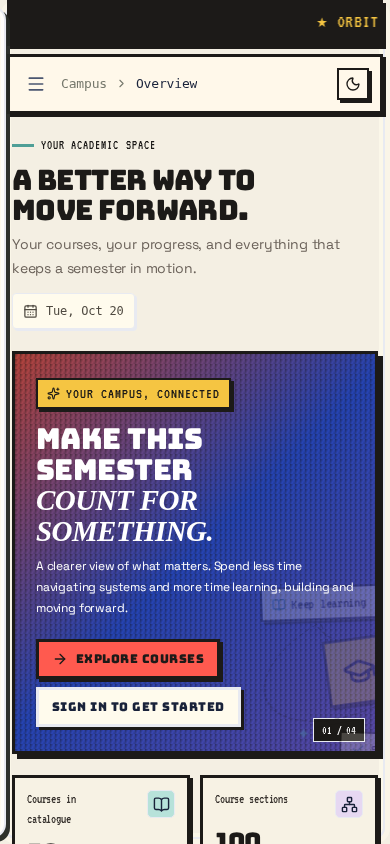
\includegraphics[width=0.43\linewidth,height=0.58\textheight,keepaspectratio]{screenshots/qa-mobile-layout-fixed.png}
\caption{Mobile layout after the responsive offset fix, captured at 390 $\times$ 844. This is targeted geometry regression evidence, not a full accessibility audit.}
\label{fig:mobile-qa}
\end{figure}

\chapter{Conclusion and next steps}
The strongest verified design property is the enrollment consistency boundary: the seat reservation and enrollment insert share a PostgreSQL transaction, and targeted concurrency tests passed in the isolated verification environment. The broader local verification also recorded a passing test suite, fresh migrations, no schema drift, a successful frontend build, API smoke checks, and stable browser navigation.

Before treating the prototype as a deployable service, the following work remains:
\begin{enumerate}
\item Add token revocation/refresh and a production identity provider; expand authentication and rate-limit abuse tests.
\item Move cache and rate-limit state to a shared backend if the application runs across multiple workers.
\item Repeat load tests over longer durations and record API, database, and load-generator resource time series.
\item Add backup/restore and failure-recovery exercises before making availability claims.
\item Implement actual data migration and replication before describing the hash-ring experiment as sharding.
\item Review crawler DNS-pinning and SSRF protections in a network-enabled test environment.
\item Add contract tests to ensure all API consumers preserve ID strings and do not coerce them to JavaScript Number.
\end{enumerate}

The results establish a verified local baseline. They do not establish production readiness. That distinction should remain explicit in demonstrations, submissions, and future benchmark reports. The report structure, figure placement, and accessible table conventions follow established technical-report guidance [1, 2].

\chapter*{References}\addcontentsline{toc}{chapter}{References}
\begin{enumerate}[label={[\arabic*]},leftmargin=2.1em,itemsep=6pt]
\item Carnegie Mellon University Robotics Institute. \textit{Technical Report Format}. Guidance on technical-report structure, readable type, figures, tables, and citations. \url{https://www.ri.cmu.edu/technical-report-format/}.
\item National Institute of Standards and Technology. \textit{NIST Technical Series Publications Author Instructions}. Guidance on report organization, plain language, accessible tables, figure captions, and references. \url{https://www.nist.gov/nist-research-library/nist-technical-series-publications-author-instructions}.
\item PostgreSQL Global Development Group. \textit{Transaction Isolation}. \url{https://www.postgresql.org/docs/16/transaction-iso.html}.
\item PostgreSQL Global Development Group. \textit{Explicit Locking}. \url{https://www.postgresql.org/docs/17/explicit-locking.html}.
\item Locust. \textit{What is Locust?}. Load-testing framework documentation. \url{https://docs.locust.io/en/2.20.2/what-is-locust.html}.
\item Carnegie Mellon University Libraries. \textit{How to Make a Science Research Poster: Design}. \url{https://guides.library.cmu.edu/scienceposters/design}.
\item Nielsen Norman Group. \textit{Visual Hierarchy in UX}. \url{https://www.nngroup.com/articles/visual-hierarchy-ux-definition/}.
\end{enumerate}

\appendix
\chapter{Reproduction checklist}
Run these commands from the \texttt{sis-app} directory with the isolated verification database available. Substitute the locally configured test password; do not commit credentials.
\begin{lstlisting}[basicstyle=\ttfamily\scriptsize,breaklines=true,breakatwhitespace=false,columns=fullflexible,frame=single,rulecolor=\color{rulegray},backgroundcolor=\color{papergray}]
export DATABASE_URL='postgresql+psycopg://sis:<local-test-password>@127.0.0.1:55432/sis_verify'
uv run alembic upgrade head
uv run alembic check
SIS_RATE_LIMIT_ENABLED=false uv run pytest -q
uv run ruff check app tests scripts migrations
cd frontend && npm run build
\end{lstlisting}

\chapter{Evidence interpretation}
\begin{itemize}
\item \textbf{Automated tests.} Evidence for the assertions exercised by the suite against the recorded database configuration.
\item \textbf{Concurrency tests.} Evidence for the tested capacity and duplicate-enrollment races, not a universal race-freedom proof.
\item \textbf{UI screenshots.} Evidence that the displayed workflows were captured from the local frontend with synthetic data, not proof of production deployment.
\item \textbf{Historical load tests.} Short local measurements that require repetition before supporting capacity estimates.
\item \textbf{Process-local components.} Functional demonstrations only, not distributed infrastructure.
\end{itemize}
\end{document}
